% \documentclass[a3paper,11pt,twoside]{thesis}
\documentclass[a4paper,palatino,11pt,twoside]{thesis}

\title{Vacuum polarization in 1+1 dimensions}
\author{Santiago Sanz Wuhl}
\department{Institut für Theoretische Physik}
\university{Universität Leipzig}

\dedication{\emph{To my family}}

% Glossaries
\newacronym[longplural={Gaussian processes}]{gp}{GP}{Gaussian process}
\newacronym{mse}{MSE}{mean squared error}

\usepackage{physics}
\usepackage{natbib}
\usepackage{amsmath}
\usepackage{amssymb}
\usepackage{mathtools}

\newcommand{\note}[1]{\textbf{\textcolor{red}{{[ #1 ]}}}}
\newcommand{\vacuum}[1]{\bra{0}#1\ket{0}}
\newcommand{\defeq}{\vcentcolon=}
\newcommand{\eqdef}{=\vcentcolon}


\begin{document}
    \startpreamble
    
    \nomenclature{$\top$}{Matrix transpose}
    
    \section*{Acknowledgements}
    I'd like to thank the following people:
    
    \newpage
    \section*{Abstract}
    Lorem ipsum dolor sit amet, consectetur adipisicing elit, sed do eiusmod tempor incididunt ut labore et dolore magna aliqua. Ut enim ad minim veniam, quis nostrud exercitation ullamco laboris nisi ut aliquip ex ea commodo consequat. Duis aute irure dolor in reprehenderit in voluptate velit esse cillum dolore eu fugiat nulla pariatur. Excepteur sint occaecat cupidatat non proident, sunt in culpa qui officia deserunt mollit anim id est laborum.
    
    \tableofcontents
    \listoffigures
    \listoftables
    
    % Change the header information for the nomenclature
    \cleardoublepage
    \markboth{\nomname}{\nomname}
    
    \printnomenclature[2cm]
    
    \stoppreamble
    
    %\chapter{Introduction}
%
%Vacuum polarization is a fundamental phenomenon of quantum field theory (QFT), one of the first theoretical predictions of quantum field theory \cite{Uehl1935}\cite{Heis1936}. It shows how the vacuum also behaves as a dynamical medium, as a dielectric with permitivity $\epsilon > 1$.
%
%For high enough external electromagnetic fields, the vacuumm will polarize inducing a non zero current density. The dependence of the current density on the applied electromagnetic field introduces non-linear terms in the Maxwell equation, leading to effects such as photon-photon scattering. Other interesting consequences of vacuum polarization is the screening behaviour of the vacuum, as (similarly to the behaviour of a classical dielectric) the polarized vacuum will act as a source for an electromagnetic field opposite to the one imposed.
%Similarly to how a dielectric breaks under strong enough external electric fields, the Schwinger mechanism predicts the generation of real electron-positron pairs. However, the particles do not have to be generated to observe the non-linear effects of the vacuum. 
%
%On another note, recent interests have arisen in the effects of considering boundary conditions for quantum field theory in the context of topological insulators.
%
%\textbf{More things to talk about}
%\begin{enumerate}
%	\item The lack of a clearly defined vacumm state both in quantum field theories on Minkowski spacetime coupled to external electromagnetic fields and in free quantum field theories in generic background spacetimes lead to a decent analogy between these two. Studying and understanding the semiclassical Klein-Gordon-Maxwell equation might be a crucial step in understanding the semiclassical Klein-Gordon-Einstein equation, or the influence of the matter fields in the gravitational fields. Understanding semiclassical gravity might be the first of many steps to understand quantum gravity.
%	\item The calcualtion of the vacuum polarization involves some ill-defined quantities, namely the product of distributions and thus require some renormalization. \cite{Ambjorn1983} do these exact calculations, as one naïvely would and get the wrong results \cite{Wendersson2022}
%	\item In this project, we redo the calculations done in \cite{Ambjorn1983}, with the correct point-split renormalization w.r.t. a Hadamard parametrix. 
%	\item We study the semiclassical approach to quantum field theory. This approach treats the background as a completely 
%\end{enumerate}
%
%These results, appearing in the study of QFTCS, will still be useful to our case. There is some parallelism to be drawn between electromagnetism and gravitation. In General Relativity, the Levi-Civita connection gives rise to the Christoffel symbols that make the covariant derivative $\nabla_\mu = \partial_\mu + \Gamma^\nu_{\mu\rho}$ covariant. In QFTCS, one is interested in solving the Einstein Field equations 
%\begin{align}
%	R_{\mu\nu} + \frac{1}{2}g_{\mu\nu}R= 8\pi\left<T_{\mu\nu} \right>_\omega,
%\end{align} 
%where the field considered interacts with the spacetime through the expectation value of its stress-energy tensor. The solutions of the Einstein Field Equations are related to the curvature tensor of the connection $R^{\lambda}_{\alpha \beta \delta} = \left[ \nabla_\alpha, \nabla_\beta \right] $.
%Similarly, in the case of electrodynamics, the connection over the $U(1)$ fiber bundle gives rise to the covariant derivative $D_\mu = \partial_\mu+ ie A_\mu $, and the dynamical equation of interest is Maxwell's equations, $\partial_\mu F^{\mu\nu}=j^{\nu}$, with $F^{\mu\nu} = [D_\mu, D_\nu]$ the curvature of the connection. We therefore argue that the results from QFTCS can be used for our case, mainly by substituting the metric covariant derivative $\nabla_\mu$ by the gauge covariant derivative $D_\mu$.
%
%\newpage

\chapter{Introduction}

Quantum field theory describes the vacuum as a state with zero occupation number in all its modes, and it is usually portrayed in the literature as a sea in which virtual particle-anti-particle pairs are constantly being created and annihilated. This picture leads to an understanding of the vacuum no longer as the absence of matter, as it is the classical assumption, but as a dynamic and fluctuating entity governed by quantum effects. cf. \cite{Peskin:1995ev, srednicki} for further discussions on the quantization of fields and their vacuum states.

One of the first theoretically studied consequences of the quantum nature of the vacuum is vacuum polarization, which arises due to the presence of external electromagnetic fields. \cite{Dirac1934} developed the expression for the charge density of the Dirac field and extended the definition to include cases where background electromagnetic fields are present. 
The polarization of the vacuum leads to a field-strength dependent charge density of the vacuum, thereby turning vacuum electrodynamics into a non-linear theory. The consequences of this effect followed shortly, as was studied by \cite{Uehl1935} and \cite{Heis1936}.

This non-linearity in Maxwell's equations causes several observable phenomena, such as corrections to the Coulomb potential \cite{Uehl1935, PhysRev.101.843},  light-by-light scattering \cite{Heis1936, ATLAS:2016pab}, 
the Lamb shift \cite{Lamb1947}, Delbrück scattering \cite{Jarl1973, ATLAS:2016pab}, and the running of the fine structure constant \cite{2017485}. These mechanisms are also relevant as observational tools, e.g. the light-by-light scattering process leading to the attenuation of high energy photons is used in measuring the Hubble constant \cite{Domí2019} (cf. \cite{Fran2021} for a review). Additionally, the presence of strong magnetic fields (e.g. near the surface of neutron stars) leads to vacuum birefringence \cite{10.1093/mnras/stw2798}, where light propagating through the vacuum experiences polarization dependent refraction. 

Furthermore, \cite{Schw51} predicts the unobserved Schwinger mechanism, in which sufficiently strong electric fields can cause a breakdown of the quantum vacuum, creating electron-positron pairs.
%In the Dirac sea picture, this can be understood as holes being allowed to quantum-tunnel through the $2mc^2$ band gap and materialez.  
This mechanism requires electric fields of the order $E_C \sim 10^{18}V/m$ (cf \cite{Dunne2009} for a review), which sets the scale at which the \textit{perturbative} approximation of 4-dimensional QED breaks down. 

The above cited calculations were performed by in the so-called semi-classical approximation, where the matter field $\phi$ is quantized, but the background electromagnetic field under which $\phi$ propagates remains classical. In this approximation, the quantum fluctuations of $\phi$ are expected to be small and it couples to the background electromagnetic field through its back reaction, i.e. the expectation value of its charge density. Thus, when studying the coupling of charged quantum Klein-Gordon fields with classical electromagnetic fields, one speaks of solving the semi-classical Klein-Gordon-Maxwell equation 
\begin{subequations}
\begin{align}
    (D_\mu D^\mu + m^2 ) \phi = 0, \\
    \partial_\mu F^{\mu \nu} = j^\nu_C + \langle j^\mu_Q \rangle,
    \label{eq:maxwell}
\end{align}
\end{subequations}
with $j^\nu_C, j^\nu_Q$ the charge currents of the classical external sources and the quantum fields, respectively.
This approximation is said to hold when the fluctuations of the quantum field do not fluctuate excessively. 
\cite{Anderson_2003} proposes quantitative tests for the validity of the semi-classical approximation.

However, as already noted by Dirac, the standard construction of quantized fields cf. \cite{Peskin:1995ev} yields a very limited  algebra of observables. 
For a $\phi$ field, this includes only linear combinations of products of fields at separate spacetime points e.g. $\phi(x) \phi(y)$.  The operators one is interested in (e.g $j^\mu_Q$), lie outside of this algebra, as they involve terms quadratic in the fields. These operators need some sense of normal ordering to be defined.

Normal ordering proceeds by defining Wick polynomials e.g. $\phi^*\phi(x)$ through the two-point correlation function of the field
\begin{align}
    \omega^{\phi ^*\phi}_0 (x, y) = \bra{0} \phi^*(x) \phi(y) \ket{0} 
\end{align}
in the following fashion
\begin{align}
    \phi^*\phi(x) = \lim_{y\to x} \phi^*(x) \phi(y) - \omega^{\phi^* \phi}_0 (x, y) \mathbf{1}.
\end{align}

In the mode expansion of the field, $\phi = \sum (a_n + a_n^\dagger)$ this corresponds to reordering of the $a_n^\dagger$ operators to the left and the $a_n$ to the right in $\phi^2(x)$.
Notice the vacuum expectation value of this operator is always zero 
\begin{align}
 \langle \phi^2(x) \rangle_0 = \bra{0}  \left( 
 \lim_{y\to x} \phi(x) \phi^*(y) - \omega^{\phi \phi^*} (x, y) \mathbf{1}
    \right) \ket{0} = 0.
\end{align}
However, this is no longer an expected behavior of the field in the presence of external charges,  as it ignores the already discussed existence of vacuum polarization. 

In defining local non-linear operators, \cite{Dirac1934} assumed that the short-distance behavior of the vacuum in the presence of external charges was the same as the vacuum in their absence, up to smooth coefficients. In modern terminology, this assumption about the behavior of the state (particularly its two-point function) is called the Hadamard condition. States obeying this condition are regarded as the only physically meaningful, which allow the evaluation of Wick polynomials. See \cite{Schl2015} for an overview of Hadamard states in the presence of external potentials.

Similar problems arise in the study of Quantum Field Theory in Curved Spacetime (QFTCS), such as the definition of non-linear observables. Other problems of similar nature, which are not discussed in this work, include the ambiguity in defining a vacuum state in generic backgrounds. Over the past decades, substantial progress has been made in describing interactions in QFTCS \cite{Brunetti1996, Brunetti2000, Sahlmann2000, Hollands_2002, Hollands_2015, Brunetti_2003}.

These developments define observables in the language of distributions via the Hadamard condition, which was elegantly reformulated in the context of the modern branch of micro-local analysis \cite{Radzikowski1996}. This formulation enables  a rigorous definition of the \textit{large momentum behavior} of a distribution in a coordinate-independent manner. Within this context, it has been possible to define normal ordering and perturbative interacting quantum field theories in essentially the same way as on Minkowski spacetime. Further discussions on the Hadamard condition can be found in \cite{Wald1977, KAY199149, Fewster_2013}.

 Vacuum polarization does not lose significance in the context of QFTCS. It has been shown to avoid particle horizons and singularities \cite{Fulling1973, Fischetti1979}, mitigate anisotropies \cite{STAROBINSKY198099, Hartle1979}, drive inflation \cite{Guth1981},  and even possibly lead to closed universes \cite{Anderson:1985vi}.

Hadamard states are relevant both in the study of QFT with background electromagnetic fields and in curved spacetimes, as the definition of renormalized local observables should depend only on geometrically constructed data, such as the Hadamard parametrix. In QFTCS, this geometry is defined by the spacetime metric,  while in QFT with background electromagnetic fields, it is determined by that of the $U(1)$  bundle over spacetime.
Additionally, in both theories one is interested in the covariance of the quantities, therefore terms such as the Christoffel symbols or the gauge potentials cannot appear.
Further readings on the relation between QED in external fields and QFTCS can be found in \cite{marecki2004quantumelectrodynamicsbackgroundexternal}.

\cite{Ambj1983} studied the behavior of the charged (complex) free Klein-Gordon field  in the presence of external charges and how the inclusion of back reaction into the calculations affected the solutions. This study initially considers the external field approximation (i.e. by neglecting the back reaction of the scalar field) and displays the appearance of a critical background electric field strength, at which the energy of certain field modes become complex, leading to runaway solutions.
Moreover, it shows that including the back reaction of the scalar field screens the external charges, stabilizing the modes and thus avoiding complex mode energies.

However, it was later shown by \cite{Schl2015, Wernersson2020}, that their calculation of the vacuum polarization is flawed,
as it failed to include the parallel transport with respect to the gauge covariant derivative in the point-splitting calculation of the vacuum polarization. \cite{Ambj1983} also reported an unexpected results: under Neumann boundary conditions, vacuum polarization exhibits anti-screening behavior. \cite{Wernersson2020} corrects both of these calculations and presents the correct way of calculating the vacuum polarization in the presence of external charges. 

In this MSc. Thesis, we use this correct prescription to calculate the vacuum polarization, and study the behavior of the quantum charged Klein-Gordon field immersed in a classical background electromagnetic field, and how backreaction affects the solutions.

%\paragraph{Divergences of the quantum fields}
%divergences of QFT appear even in the consideration of the simplest theories. In the quantization of the free real scalar field, divergences appear when one tries to calculate any non-linear polynomial on the field, due to the presence of $a a^\dagger$ terms in the mode expansion of the field. In the absence of background electromagnetic field, this is usually dealt with by defining these observables through normal ordering, i.e. $\mathcal{O}(\phi) \to :\mathcal{O}(\phi):$. In this prescription, evaluation of an observable $:\mathcal{O}(\phi):$ in the state $\omega$ is defined by
%$$\left<: \mathcal{O}(\phi):\right>_\Omega = \bra{\Omega}  \mathcal{O}(\phi) \ket{\Omega}  - \bra{0}  \mathcal{O}(\phi) \ket{0}.$$
%this prescription is in itself very powerful in the context of QFT in the absence of background fields. 
%
%however, one of the key properties of normal ordering is yielding $\left<: \mathcal{O}(\phi):\right>_0=0$ for the vacuum state. This is no longer a desired behavior in the presence of background electromagnetic fields, as this would predict the vacuum polarization to be always zero, and is existence is already discussed.
%\cite{Dirac1934} proceeded by assuming that the vacuum state $\ket{0}_A$ in the presence of an electromagnetic field $A$ has the same short-range behavior as the $\ket{0}$ state in the absence of background electromagnetic field, up to smooth coefficients. That the vacuum state of the field is of this form is called the Hadamard condition, and the class of Hadamard states (i.e. states which verify the Hadamard condition) are usually said to be the only physically relevant states. 
%
%a \note{(quasi free?)} state is said to be Hadamard if its two-point function $w(x, x')$ is of the form 
%\begin{align}
%   w^{\phi \phi^*}_\Omega (x, x') = \bra{\Omega} \phi(x) \phi^*(x') \ket{\Omega} =  H^{\phi \phi^*}(x, x') + R^{\phi \phi^*}_\Omega(x, x').
%\end{align}
%here $H^{\phi \phi^*}(x, x')$, the Hadamard parametrix, is a state-independent bi-solution to the Klein-Gordon equation, with a divergence structure as $x' \to x$ very similar to that of the two-point function of the vacuum state in the absence of background electromagnetic fields. $R^{\phi \phi^*}_\Omega(x, x')$ is a smooth function that contains the dependence on the state $\Omega$.
%
%The Hadamard parametrix is calculated by integrating the Klein-Gordon equation along the geodesic that joins $x$, $x'$ (straight lines in flat spacetime), and by parallelly transporting the parametrix with respect to the gauge covariant derivative induced by the connection over the $U(1)$ principal bundle defined over the spacetime.
%\cite{Ambj1983} calculates the vacuum polarization without the inclusion of this parallel transport, which leads to a wrong expression as was shown by \cite{Schl2015, Wernersson2020}.


\newpage
\section*{Notation and conventions}

Throughout this thesis, we use natural units $\hbar = c = 1$. We work on flat 1+1 dimensional Minkowski spacetime, with the `mostly negative' metric (+, -). $x$ will usually denote an event in the spacetime, with $x^{0}$, $x^{1}$ its time and spatial components, respectively. The partial derivatives with respect to these coordinates will then be 
\begin{align}
\partial_\mu := 	\frac{\partial}{\partial x^{\mu}}.
\end{align}
We also use a different coordinate choice,  which will describe the spacetime with coordinates $t$, $z$ for the time and spatial components, respectively. Similary 
\begin{align}
	\partial_t:= 	\frac{\partial}{\partial t}, \hspace{0.2cm}  \hfill
\partial_z:= 	\frac{\partial}{\partial z}.
\end{align}

Unless noted otherwise, Einstein's summation convention is assumed, i.e. 
\begin{align}
	a_\mu b^{\mu}= \sum a_\mu b^{\mu}.
\end{align}




    \chapter{Preliminaries}

%\paragraph{Why this chapter?}
%This chapter appears because in the following chapter I calculate the expression of the expectation value of the charge density through Hadamard point-split renormalization
%
%\paragraph{What is this chapter's end goal?}
%Derive an expression for Hadamard point split renormalization.
%
%\paragraph{Why is Hadamard point split renormalization needed?}
%Because we want to solve 
%\begin{align}
%	\partial_\nu F^{\mu\nu} = \left<j^\mu \right>_\omega
%\end{align}
%w.r.t. some state $\omega$, and the RHS of this equation is ill-defined due to the appearance of products of fields. Hadamard point splitting renormalization defines the expectation value of these terms in mathematically precise way, yielding finite values and assuring gauge invariance of the calculated expectation values.
%
%\paragraph{What do we need for this?}
%\begin{enumerate}
%	\item The phase space
%		\begin{enumerate}
%			\item Symplectic space and time evolution in the space.
%			\item Isomorphism between phase space $\mathcal{M}$ and solution space  $\mathcal{S}$ .
%			\item Classical observables $f\mathcal{C}^{\infty}_0 (S)$ form a vector space. Can be given algebraic structure via $ \{f, g\} = \Omega^{ab}\nabla_af\nabla_bg$
%			\item Quantization of the phase space. Quantum observables are self-adjoint operators on $\mathcal{S}$. Quantization map $\,\hat{}:\mathcal{O}\to \hat{\mathcal{O}}$, such that for any pair of classical observables we have
%			\begin{align}
%				[\hat{f}, \hat{g}] = i \hat{\{f, g\} },
%			\end{align}
%			with $[\,,]$ the commutator and $\{\,,\} $ the Poisson bracket.
%		\item Define observables through points in the manifold: $\forall y \in \mathcal{M}, \Omega(y, \cdot ) $ defines a (classical) observable on $\mathcal{M}$. Quantize by requiring 
%		\begin{align}
%		[\hat{\Omega}(y_1,\cdot ), \hat{\Omega}(y_2, \cdot )] = -i \Omega(y_1, y_2) I,
%		\end{align}
%		which is the usual quantization.
%	\item Quantum theory of harmonic oscillators. Annihilation operator 
%	\begin{align}
%		a = \sqrt{\frac{\omega}{2}} q + \sqrt{\frac{1}{2\omega}} p
%	\end{align}
%		Its Heisenberg representation 
%		\begin{align}
%			a_H(t) = U_t^{-1}aU_t = e^{-i\omega t} a,
%		\end{align} 
%		leads to the Heisenberg representation of the position operator 
%		\begin{align}
%			q_H = \sqrt{\frac{1}{2\omega}}  (a_H + a_H^{\dagger}) = \sqrt{\frac{1}{2\omega}}  \left( e^{-i\omega t} a + e^{i\omega t} a^\dagger \right) .
%		\end{align}
%		The annihilation operator is the positive frequency part of the position operator.
%		\end{enumerate}
%	\item Define One-particle Hilbert spaces $\mathcal{H}\subset \mathcal{S}$ as the space of positive frequency solutions 
%	\begin{align}
%		q_i = \alpha_i e^{-i\omega_i t}.
%	\end{align}
%	 $\mathcal{H}$ is a Hilbert space (can define an inner product given by the symplectic form $(y_1, y_2) = -i \Omega(\overline{y_1}, y_2)$. Construct its (symmetric) Fock space $\mathcal{F}_s(\mathcal{H})$. Choose  the (normalized w.r.t. ( , )) solution to the classical EOM $\xi_i\in\mathcal{H}$ s.t. only the $i$-th oscillator is excited. Therefore define the q, p observables to be 
%	 \begin{align}
%	 	q_{iH}(t) =  \xi_i(t) a_i + \overline{\xi_i}(t) a^\dagger, p_{iH}  = \dot q_{iH}
%	 \end{align}
% \item Construct the negative frequency solution space as $\mathcal{\overline{H}}$. Define $K$ as the projector $K:\mathcal{S}\to \mathcal{H}$ (and consequently $\overline{K}:\mathcal{S}\to \mathcal{\overline{H}}$). 
% \begin{align}
% 	\forall y \in \mathcal{S}, \hat{\Omega}_H (y,\cdot ) := ia (\overline{Ky}) - ia^\dagger (Ky)
% \end{align}
%	\item Klein-Gordon in flat spacetime. Linearity of KG equation allows to study the system as infinite harmonic oscillators, decoupled. Define momentum through the lagrangian $\pi = \frac{\delta S}{\delta \dot\phi} = \dot \phi$. KG is initial value problem, define  $\mathcal{M}$ as the (compact) Cauchy data defined over a Cauchy surface $\Sigma_0$
%	\begin{align}
%		\mathcal{M} := \{ [\phi, \pi]  \in C_0^{\infty}(\Sigma)\times  C_0^\infty(\Sigma)  \} 
%	\end{align}
%	Every point in $\mathcal{M}$ defines a single solution to the KG equation. There is therefore a direct identification with the solution space  $\mathcal{S}$.
%	The symplectic structure on  $\mathcal{S}$ 
%	\begin{align}
%		\Omega([\phi_1, \pi_1],[\phi_2, \pi_2]) = \int_{\Sigma}^{}  d^3x (\pi_1\phi_2 - \pi_2\phi_1).
%	\end{align}
%	\item Test functions. 
%	Given any element $f\in C_0^{\infty} (M) = \mathcal{T}$ (in flat spacetime case, $M=\mathbb{R}^{4}$,) define its advanced and retarded propagators as 
%	\begin{align}
%		(\partial_a\partial^{a}-m^2) (Af) = f, \,
%		(\partial_a\partial^{a}-m^2) (Rf) = f,
%	\end{align}
%	such that  $\text{supp}(Af) = J^{-}(\text{supp}(f))$, $\text{supp}(Rf) = J^{+}(\text{supp}(f))$. Define the causal propagator $Ef = Af-Rf$. $E:\mathcal{T}\to \mathcal{S}$ defines an onto, non degenerate map. Also verifies that 
%	\begin{align}
%		\int \psi f d^{4}x = \Omega(Ef, \psi), \forall \psi \in \mathcal{S}, f \in \mathcal{T}.
%	\end{align}
%	This allows one to define, for each $f\in \mathcal{T}$ the field as an averaging of the solution to KG weighted by $f$. 
%	\begin{align}
%		\hat{\phi}(f) = \hat{\Omega}(Ef, \cdot ) = ia(\overline{K(Ef)} - ia^\dagger (K(Ef))
%	\end{align}
%	is then to be understood as the weighted spacetime average of the field operator representing the field at spacetime point $x$.
%	$ \overline{\phi}$ is an operator-valued distribution, and solves the KG equation in the distributional sense ,
%	\begin{align}
%	KG \hat{\phi}(f) = 	\hat{\phi}(KG(f)) = \hat{\Omega}(E(KG(f)), \cdot  ) = 0
%	\end{align}
%Choosing the vacuum state as that which verifies $a_{\textbf{k}}\ket{0}=0$  for all $\textbf{k}$, then the vacuum two point function is defined as 
%\begin{align}
%	w(f, g) = \vacuum{\hat{\phi}(f) \hat{\phi}(g) }.
%\end{align}
%With the definition of the field being averaged weighted by $f$, then 
%\begin{align}
%	w(f, g) &= \vacuum{\int_{M}^{} \phi(x) f(x) d^{4}x  \int_{M}^{}  \phi(y)g(y)d^4y  } \\
%		&= \int_{M\times M}^{}  \vacuum{\phi(x) \phi(y)} f(x)f(y) d^{4} xd^{4} y.
%\end{align}
%This expression defines the distributional notation 
%\begin{align}
%	w(x, y)  = \vacuum{\phi(x) \phi(y)},
%\end{align}
%so that two point functions can be understood as a bi-solution to the Klein-Gordon equation.
%	\item We are interested in calculating the charge current density  of the Klein-Gordon field
%	\begin{align}
%		j^{\mu} = ie \left( (D^\mu \phi)^* \phi - \phi^* D^{\mu}\phi \right) .
%	\end{align}
%	This observable contains products of fields, whose distributional nature automatically makes its expectation value ill-defined. To calculate this quantity, it needs to be redefined.
%
%	In attempting to directly calculate this expectation value, one finds that the terms containing $a a^{\dagger}$ in the mode expansion of the 'field' $\phi^2$ yield a diverging expectation value, with all other terms vanishing (in a real field. In a complex field the $b b^\dagger$ will also contribute to an infinite expectation value.) In QFT in flat spacetime one proceeds by 'normal ordering' i.e. by moving the creation operators to the right and the annihilation operators to the left, or more precisely by defining $ \left< :a a^\dagger: \right>_\omega = \left< a^\dagger a \right>_\omega$. Notice how this prescription implies (in the abscence of external electric fields)
%	\begin{align}
%		\vacuum{:j^{\mu}:} = 0,	
%	\end{align}
%	as one would expect.
%
%	Evaluating $ \left<\phi(x)^2 \right>_\omega$ for a state $\omega$ is problematic, but the two point function is well defined as a bi-solution to the Klein-Gordon equation. This distribution will not be smooth in the limit $x'\to x$, but with suitably chosen states the difference
%	\begin{align}
%		F(x, y) = \left<\phi(x)\phi(y) \right>_\omega - \vacuum{\phi(x)\phi(y)}
%	\end{align}
%	is.
%	We therefore define the expectation value of terms quadratic in the field through a point-splitting procedure 
%	\begin{align}
%\left<\phi^*(x)\phi(x) \right> = \lim_{x' \to x} F(x, x').
%	\end{align}
%
%	This definition can be extended through linearity to our quantity of interest 
%	\begin{align}
%		\left<j^\mu \right>_\omega := \frac{ie}{2}\lim_{x' \to x}  \left( D^*_\mu F(x, x') - D'_\mu F(x, x') \right) ,
%	\end{align}
%	with $D_\mu^* = \partial_\mu - ieA_\mu$ and $D'$ the derivative over primed variables. $j^{\mu}$ should be parallely transported with respect to the gauge covariant derivative.
%
%	This prescription coincides with the normal ordering prescription on flat spacetimes with no background electromagnetic field, but considering curved spacetimes or background electromagnetic fields (i.e. connections over $U(1)$ with curvature) takes away having a preferred choice of a vacuum state, and therefore defining these expectation values through the vacuum state as above becomes problematic. Even when the vacuum state can be defined, we do not expect  
%	\begin{align}
%		\vacuum{j_\mu} = 0
%	\end{align}
%	with a non zero background electromagnetic background.
%
%	The prescription above, however, defines the difference of these expectation values between states. In this sense, the difference 
%	\begin{align}
%		\left<j_\mu \right>_1 -
%		\left<j_\mu \right>_2 
%	\end{align} is smooth for two states $\omega_1, \omega_2$.
%
%	We can develop this idea to come up with a formal definition of the difference between expectation values on different states. To this end, we list some the properties that we expect from $ \left<j_\mu \right>$. The full list can be found in \cite{Wald1994}. 
%	\begin{enumerate}
%		\item The difference between states $ \left<j_\mu \right>_1 - \left<j_\mu \right>_2$ to be smooth whenever the difference $\left<\phi(x)\phi(x') \right>_1- \left<\phi(x)\phi(x') \right>_2$ is a smooth function.
%		\item  $D_\mu\left<j^\mu \right>_\omega=0$ for any state $\omega$,
%		\item $\vacuum{j_\mu}  = 0$ in flat spacetime with no background electromagnetic field.
%	\end{enumerate}
%
%From property (a), two different definitions of the expectation value $\left<j_\mu \right>_\omega$, $\left<\overline{j}_\mu \right>_\omega$ must obey 
%\begin{align}
%	\left<j_\mu \right>_1-
%	\left<j_\mu \right>_2 = 
%	\left<\overline{j}_\mu \right>_1-
%	\left<\overline{j}_\mu \right>_2,
%\end{align}
%and therefore the quantity  $\mathcal{J}_\mu = \left<j_\mu \right>_1-\left<\overline{j}_\mu \right>_1$ is independent of the state considered. This, with a certain additional property of the expectation value $\left<j_\mu \right>_\omega$ implies that $\mathcal{J}_\mu(x)$ is only dependent locally. Finally, (b) imply that  $\mathcal{J}_\mu$  is conserved and (c) that for no background electromagnetic field, $\mathcal{J}_\mu=0$. 
%
%The prescription for $\left<j_\mu \right>_\omega$ can be shown to be unique up to local background field terms, but not necessarily existent. The prescription can be built from "point-splitting" so that for any $\left<\phi(x)\phi(x') \right>$ a bi-solution to the Klein-Gordon equation $H(x, x')$ is subtracted. Through this prescription, $\left<j_\mu \right>_\omega$ obeys the required properties, as long as $H(x, x')$ exists. A proof of the uniqueness of the definition of non linear observables can be found in \cite{1977Wald}.
%
%We choose an ansatz for $H(x, x')$ such that it shares a singularity structurure with vacuum two point function of the scalar field on flat (even) $n$ dimensional spacetime with no background electromagnetic field, up to smooth coefficients $V_k$
%\begin{align}
%	H(x, x') = \sum_{k}^{\infty} V_kT_k + W(x, x'),
%\end{align}
%with 
%\begin{align}
%	T_k = 
%	\begin{cases}
%		\frac{( \frac{n}{2} - 2 - k)!}{2 (2\pi)^{n/2} }\sigma_\varepsilon ^{- (\frac{n}{2}-1-k)} & k \leq \frac{n}{2}-2 \\
%	-\frac{1}{2 (2\pi)^{n/2} ( k-\frac{n}{2}+1) }(-\sigma) ^{-k - \frac{n}{2} + 1}\log\left(\sigma_\varepsilon  \right)  & k > \frac{n}{2} - 2,
%	\end{cases}
%\end{align}
%where $\sigma(x, x')$ is the geodesic distance from $x$ to $x'$ (which in Minkowski spacetime corresponds to  
%$
%	\sigma(x, x') = (x - x')^2,
%	$
%	and 
%	\begin{align}
%		\sigma_\varepsilon = \sigma + 2i\varepsilon(t-t') + \varepsilon ^2.
%	\end{align}
%	$t, t'$ are the time coordinates of $x, x'$ given by an appropiate choice of a time coordinate function. It is also understood that the limit $\varepsilon \to 0^+$ should be taken after applying this to test functions.
%	The coefficients $V_k$ and the function $W$ are to be obtained by solving $\mathcal{K} H(x, x)=0$. This equation gives an ordinary differential equations for each of the $V_k$ that should be solved with the initial condition $V_0(x, x')=1$, and integrated along the geodesics (straight lines) joining $x$ and $x'$.
%
%	With a working prescription of the expectation value of non-linear terms on the field, we can finally formally define 
%	\begin{align}
%		\left<D_\alpha D^*_\beta \phi(x) \phi^*(x) \right> :=  \lim_{x' \to x} D_\alpha D'^*_\beta \left( \left<\phi(x) \phi^*(x')  \right> - H(x,x') \right),
%	\end{align}
%	with $\alpha, \beta$ symmetrized multiindices.
%
%
%
%\end{enumerate}


%The back-reaction of a field generally appears in the context of the semiclassical approach to quantum field theory. This considers a classical background, and the coupling of a quantum field to said background through the expectation value of the charge current defined by the dynamical law considered. The typical case of study of the back-reaction problem is semiclassical gravity, i.e. the coupling of a scalar field $\phi$ to a classical background spacetime metric. This is mediated by semiclassical Einstein equations
%\begin{align}
%	\begin{split}
%		G_{\mu\nu}&= 8 \pi \left<T_{\mu\nu} \right>,\\
%		%R_{\mu\nu} - \frac{1}{2}R g_{\mu\nu} - \Lambda g_{\mu\nu} &= 8 \pi T_{\mu\nu} ,\\
%		T_{\mu \nu } &=  \nabla _{\mu} \phi ^* \nabla _{\nu}\phi - \frac{1}{2}g_{\mu\nu} \left( \nabla _{\beta}\phi^*\nabla ^{\beta}\phi + m^2 \phi^*\phi\right).
%	\end{split}
%	\label{eq:semiclassical-gravity}
%\end{align}
%In this thesis we study however semiclassical electrodynamics, i.e. the coupling of the scalar field to a background classical electromagnetic field, mediated by the semiclassical Maxwell equations
%\begin{align}
%	\begin{split}
%		\partial_\nu F^{ \mu\nu}&=   \left<j ^ \mu \right>,\\
%		j^\mu &=ie \left( ( D^{\mu} \phi)^{*} \phi- \phi^{*}D^\mu \phi \right) .
%	\end{split}
%	\label{eq:semiclassical-electrodynamics}
%\end{align}
%The fields are to be seen as distributions smeared over test functions. This implies that these expectation values are ill-defined, as they involve evaluating a pointwise product of distributions. The expectation values of these operator fields need to be therefore redefined.
%
%The following chapter presents basic theory, context and techniques from QFTCS that are going to be used in following chapters to calculate the quantities defined above, and it is not meant as an instructive text. A more detailed introduction to these topics can be found in \cite{QFTCS, Wald1994}. Eventhough the techniques developed in the mentioned texts present a very different physical context to the one of interest for this thesis (semiclassical gravity is a QFT on a curved spacetime, where as semiclassical electrodynamics studies QFT under a curved connection in the $U(1)$ bundle over flat spacetime,) the mathematical framework developed can still be used under the substitution of the metric covariant derivative $ \nabla _\mu$ with the gauge covariant derivative $D_\mu$.
%
%AQFT differs from the usual construction of QFTCS in that instead of constructing an operator algebra from the Hilbert space, one begins from an observable algebra $\mathcal{A}$ and a state $\omega: \mathcal{A}\to \mathbb{C}$, and constructs a Hilbert space from these two objects. These approach presents the advantages of taking a more general perspective, which allows one to circumvent certain problems QFTCS presents, such as unitary inequivalence of representations of the same quantum field theory (with some techni

%Eventhough the physical contexts for semiclassical gravity and semiclassical electrodynamics are mediated by very different physical laws, the mathematical framework for these two problems allows for the utilisation of the results from \cite{QFTCS, Wald1994} to our study of the Klein-Gordon-Maxwell equations. The similarities lie in the substitution of the metric covariant derivative $\nabla_\mu$ with the gauge covariant derivative $D_\mu$, and its consequences, such as parallel transport being defined through its corresponding covariant derivative.

%\section{The quantization of the phase space}
%
%The configuration space $\mathcal{Q}$ of a classical system with $n$ degrees of freedom is an $n$ dimensional manifold which as the name implies, collects all possible configurations of the system. Given $\mathcal{Q}$, its phase space $\mathcal{P}$ will be a $2n$ dimensional manifold, and it can be constructed as the cotangent bundle $T^*\mathcal{Q}$, i.e. each $q \in\mathcal{Q}$ and its attached cotangent space $T^*_q \mathcal{Q}$. 
%
%With the definition of a Hamiltonian function $H$ over the phase space $\mathcal{P}$, dynamical evolution is given by Hamilton's equations (assuming coordinates $q_i$ for $q\in\mathcal{Q}$ and $p_i$ for  $p\in T^*_q \mathcal{Q}$)
%\begin{align}
%	\dot q_i &= \frac{\partial H}{\partial p_i} \\
%	\dot p_i &= -\frac{\partial H}{\partial q_i}
%\end{align}
%where a dot denotes time derivative. This can be written more succintly as 
%\begin{align}
%	\dot y = \Omega^{} \frac{\partial H}{\partial y},
%\end{align}
%with \note{canonical coordinates} $y=(q_1, \ldots, q_n, p_1,  \ldots p_n) \in \mathcal{P}$ and
%\begin{align}
%	\Omega^{ji}  = \begin{pmatrix} 0 & I_n \\ -I_n& 0  \end{pmatrix}.
%\end{align} 
%
%This can be formulated in the more general language of Hamiltonian mechanics, in which the essential mathematical structure needed is given by the phase space $\mathcal{P}$ and a symplectic form $\Omega_{ab}$, i.e. nondegenerate, closed, 2-form on $\mathcal{P}$. The symplectic form $\Omega_{ab}$ presents an inverse symplectic form $\Omega^{ab}$,  which satisfies $\Omega_{ab}\Omega^{bc} = \delta_a^c$. The Hamiltonian function $H: \mathcal{P} \to \mathbb{R}$ dictates the dynamical evolution of the system, as the integral curves of the vector field 
%\begin{align}
%	h^{a} = \Omega^{ab}\nabla_b H.
%\end{align}
%This allows us to identify the solution space $\mathcal{S}$ of the equations of motion, i.e. each point $y \in \mathcal{P}$  gives rise to a solution $y(t)\in \mathcal{S}$ of the dynamical equations of motion such that $y(0) = y$.
%
%Classical observables  are defined as real valued functions over the phase space. The set of observables presents an (infinite dimensional) vector space structure, and it can be given an algebraic structure through the Poisson bracket 
%\begin{align}
%	\{f, g\} = \Omega^{ab}\nabla_a f \nabla_b g.
%\end{align}
%The Poisson bracket presents the usual results 
%\begin{align}
%	\{q_{\mu}, q_{\nu}\}   =
%	\{p_{\mu}, p_{\nu}\}   = 0 \\
%	\{q_{\mu}, p_{\nu}\}   = \delta_{\mu\nu} 
%\end{align} 



%By assuming the ansatz 
%equation \eqref{eq:TDKGE} turns into 
%\begin{align}
%	\left( -(\omega_n - eA_0)^2 + D_iD^i + m^2 \right) \phi_n(\textbf{x}) =   0
%\end{align}
%
%\begin{align}
%	 \mathcal{F}(\mathcal{H}) = \oplus_{n=0}^\infty \mathcal{H}^{\otimes n}
%\end{align}

\section{Quantization of the free complex scalar field}

The free Klein-Gordon equation for a complex field $\phi$ in two spacetime dimensions is
\begin{align}
	(D(t, x)_\mu D(t, x)^{\mu} + m^2)\phi(t, x) = 0,
	\label{eq:Klein-Gordon}
	%\partial_\nu F^{\nu\mu} &= \left<j^{\mu} \right>.
\end{align}
with $D(t, x)_\mu = \partial_\mu +i e A(t, x)_\mu$ the gauge covariant derivative  and $D(t, x)^\mu = \eta^{\mu\nu}D(t, x)_\nu$, with $\eta$ the 2-dimensional Minkowski metric. We drop from now on the explicit dependence of the derivative with the spacetime coordinates.

The general solution to equation \eqref{eq:Klein-Gordon} is 
\begin{align}
	\phi(t, x) = \sum_{n>0}^{} a_n \phi_n (x) e^{-i\Omega_n t}
+\sum_{n<0}^{} b^*_n \phi_n (x) e^{-i\Omega_n t},
\end{align}
with $a_n, b_n$ complex coefficients depending on $n $, and $\phi_n$ solutions to the time independent Klein-Gordon equation
\begin{align}
	\left[ \left( \Omega_n - eA_0 \right)^2 + \partial_1^2 - m^2  \right] \phi_n(x) = 0,
\end{align}
with $\Omega_n$ gauge dependent energy parameters that are calculated when applying the boundary conditions $\phi$ is subjected to. The $\phi_n$ are orthonormal with respect to the inner product 
\begin{align}
	(\phi_n, \phi_m) = \int_{\mathbb{R}}^{} \left( D_0\phi_n(x) \phi_m(x)^* - D_0^*\phi_n(x)^* \phi_m(x) \right) dx
\end{align}
and obey the completeness relation
\begin{align}
	i \sum_{n=-\infty}^{\infty} \phi_n(t, x') \partial_0 \phi_n(t, x) - \phi_n(t, x) \partial_0 \phi_n(t, x') = \delta ( x - x').
\end{align}

The canonical momentum $\pi$ associated to the field $\phi$ is calculated as
\begin{align}
	\pi(x) = D_0^*\phi^*= i\sum_{n>0}^{} a^*_n(\Omega_n - eA_0)\phi^*(x) e^{i\Omega_n t}
+ i\sum_{n<0}^{} b_n(\Omega_n - eA_0)\phi^*(x) e^{i\Omega_n t},
\end{align}
and equivalently for the momentum $\pi^*$ associated to $\phi^*$ is  
\begin{align}
	\pi^*(x) = D_0\phi= -i\sum_{n>0}^{} a_n(\Omega_n - eA_0)\phi(x) e^{-i\Omega_n t}
- i\sum_{n<0}^{} b_n^*(\Omega_n - eA_0)\phi(x) e^{-i\Omega_n t}.
\end{align}

Canonical quantization proceeds by promoting the classical fields $\phi, \pi$ to operators on the state Hilbert space obeying the same-time commutation relations 
\begin{align}
	[\phi(t, x), \pi(t, y)] = 
	[\phi^*(t, x), \pi^*(t, y)] = i \delta(x-y).
\end{align}
The imposition of these commutation relations, together with the orthonormality and completeness condition, imply that the quantum operators corresponding to the classical coefficients $a_n$, $b_n$ are the ladder operators obeying the commutation relations
\begin{align}
	[a_n, a_m^\dagger] &= [b_n, b_m^\dagger]= \delta_{nm}, \\
	[a_n, a_m] = [b_n, b_m]&= 
	[a_n, b_m] = [a_n, b^\dagger_m]=  0.
\end{align}
The ladder operators, in particular the annihilation operators $a_n, b_n $ define the vacuum state as that element of the Hilbert space of states which obeys 
\begin{align}
	a_n \ket{0} = b_n \ket{0} = 0.
\end{align}
%We proceed in the construction of quantum field theory as the quantization of a classical field theory. Therefore, consider the lagrangian of the complex free field
%\begin{align}
%	\mathcal{L} = \partial_\mu\phi^* \partial_\mu\phi + m^2\phi^*\phi.
%\end{align}
%From the lagrangian one can calculate the equations of movement of the field , namely the Klein-Gordon equation
%\begin{align}
%	\left( \partial_\mu\partial^\mu + m^2 \right) 	\phi = 0.
%\end{align}
%One also defines the canonical momentum associated to the scalar field $\pi = \frac{\partial \mathcal{L}}{\partial \partial_0\phi}  =  \left(\partial_0 \phi  \right) ^*$. One also calculates the Hamiltonian density of the Klein-Gordon field as the Legendre transform of the Lagrangian
%\begin{align}
%	H = \frac{1}{2}\pi^* \pi + \frac{1}{2} \left( \nabla  \phi\right) ^*\left(  \nabla \phi \right) + m^2\phi^*\phi.
%\end{align}
%
%Linearity of the Klein-Gordon equation allows one to decompose it into a mode equation by assuming the ansatz 
%\begin{align}
%	\phi(t, x) = \sum_{}^{} a_n \phi_n e^{-i\omega_nt}
%+	 \sum_{}^{} b^*_n \phi_n e^{+i\omega_nt}.
%\end{align}
%The expansion of $\phi$ presents the two sets of coefficients  $a_n$, $b_n$ which arise from the added degrees of freedom due to  $\phi$ being a  complex field.
%

One also talks about the two two-point functions for a particular state $\chi$\footnote{The two point functions are also defined distributionally by 
\begin{align}
	w^{\phi \phi^*}(f, g) = \bra{\Omega} \phi(f)\phi^*(g) \ket{\Omega} = \int_{\mathbb{R}^2\times \mathbb{R}^2}^{}  w^{\phi\phi^*}_\Omega(x, x') f(x) g(x')dx dx'
\end{align}}
\begin{align}
	w_\chi^{\phi \phi^*}(t, x; t', x') &= \bra{\chi} \phi(t, x) \phi^*(t', x') \ket{\chi}  \\
	w_\chi^{\phi^* \phi}(t, x; t', x') &= \bra{\chi} \phi^*(t, x) \phi(t', x') \ket{\chi}.
\end{align}
In particular for the vacuum state, they present the following form
\begin{align}
	w_0^{\phi_n \phi_n^*}(t, x; t', x') &= \sum_{n>0}^{}  \phi_n(x)\phi_n^*(x') e^{-i\Omega_n(t-t')} \\
		w_0^{\phi_n^*\phi_n }(t, x; t', x') &= \sum_{n<0}^{}  \phi_n(x)\phi_n^*(x') e^{i\Omega_n(t-t')}.
\end{align}
The two-point function is a bi-solution of the Klein-Gordon equation
\begin{align}
	\mathcal{K}w_\chi^{\phi \phi^*}(t, x; t', x')  
	= \mathcal{K'} w_\chi^{\phi \phi^*}(t, x; t', x')   = 0.
\end{align}
In the previous equation $\mathcal{K} = D_\mu D^{\mu} + m^2$ the Klein-Gordon operator, and $\mathcal{K'}$ the Klein-Gordon operator acting on the variables $(t', x')$.

Finally, measurement of a linear observable $\mathcal{O}(\phi)$ $\phi$ is done by taking its expectation value with respect to some state 
\begin{align}
	\left< \mathcal{O}(\phi) \right>_\chi =\bra{\chi} \mathcal{O}\phi \ket{\chi} .
\end{align}
Observables $\mathcal{O}(\phi)$ non-linear on the fields involve taking the product of the distributions $\phi$. This operation is a priori ill-defined and its proper mathematical definition is dealt with in the next section.

%\paragraph{Schrödinger vs. Heisenberg picture}
%In non-relativistic quantum mechanics (this can also be done in QFT, but it is non-standard), the usual way of studying solutions to the Schrödinger equation is using the Schrödinger picture.
%The Schrödinger picture means that solutions to the Schrödinger equation 
%\begin{align}
%	i\hbar \partial_t \psi(t, \textbf{x}) = H \psi(t, \textbf{x})
%\end{align}
%evolve in time as follows 
%\begin{align}
%	\psi(t, \textbf{x}) = e^{-iH (t-t_0)} \psi(t_0, \textbf{x}),
%\end{align}
%i.e. it focuses in the study of the time evolution of the wave function, where the operators remain "constant" in time. In this picture, the evaluation expectation values of some observable in the Schrödinger picture $\mathcal{O}_S$ and its evolution in time goes as 
%\begin{align}
%	\bra{\phi(t, \textbf{x})} \mathcal{O}_S \ket{\phi(t, \textbf{x})}  = 
%	\bra{\phi(t_0, \textbf{x})} e^{iH(t-t_0)} \mathcal{O}_S e^{-iH(t-t_0)} \ket{\phi(t_0, \textbf{x})} .
%	\label{eq:time-evolution-in-the-schrodinger-picture}
%\end{align}
%One might equivalently work in the Heisenberg picture, in which the study focuses on the time evolution of the operators, and the vectors are time-independent. By observing \eqref{eq:time-evolution-in-the-schrodinger-picture}, the operator $\mathcal{O}$ in the Heisenberg picture is defined as 
%\begin{align}
%	\mathcal{O}_H = e^{iH(t-t_0)} O_S e^{-iH(t-t_0)},
%\end{align}
%and differentiation of this expression with respect to time yields the equivalent time evolution equation for the operator $\mathcal{O}$ in the Heisenberg equation 
%\begin{align}
%		\frac{d\mathcal{O}_H}{dt} = i[H, \mathcal{O}_H].
%\end{align}
%

%When solved with compactly supported Cauchy data $\left(\left. \phi\right|_\Sigma, \left. n^{\mu}D_\mu\phi \right|_\Sigma\right)$, with $\Sigma$ a space-like hypersurface (typically a constant-$t$ surface) and $n$ a unit vector orthogonal to $\Sigma$, the global hyperbolicity of Minkowski spacetime ensures that this problem is well posed.
%		The collection of all possible smooth $\phi$ with compactly supported Cauchy data forms the configuration space $\mathcal{C}$. From $\mathcal{C}$ one constructs the phase space $\mathcal{P} = T^*\mathcal{C}$, as its cotangent space. The elements of $\mathcal{P}$ are the points $(\phi, \pi)$, with $\pi=D_0^*\phi^*$ the canonical conjugate of the field $\phi$. Points in the phase space correspond to initial conditions for the Klein-Gordon equation on the Cauchy surface $\Sigma.$
%		$\mathcal{P}$ can be endowed with symplectic structure with the symplectic\footnote{Bilinear, antisymmetric} form
%		\begin{align}
%			\sigma((\phi_1, \pi_1), (\phi_2, \pi_2)) = i \int_\Sigma \left( \pi_1^* \phi_2^*- \pi_2\phi_1 \right) d\Sigma.
%		\end{align}
%		It is not difficult to prove that $\sigma$ is a time evolution invariant if $\phi_1$, $\phi_2$ are solutions to the Klein-Gordon equation, as long as they are compactly supprted. \note{Prove this? In appendix?}
%	
%The solution space  $\mathcal{S}$ is the space of all smooth solutions to the Klein-Gordon equation. As the initial data fully determines a solution to the Klein-Gordon equation, each solution corresponds to a point in phase space and therefore $\mathcal{S}$ can be identified with $\mathcal{P}$.
%$\mathcal{S}$ can be given Hilbert space structure as follows: 
%\begin{enumerate}
%	\item Define the subspace $\mathcal{S}_+$ of positive frequency solutions. In this subspace the symplectic product can be made positive definite.
%	\item Define a Hermitian inner product in this subspace 
%	\begin{align}
%		(\phi_1, \phi_2) = i\sigma(\phi_1^*, \phi_2), \,\,\, \phi_1, \phi_2 \in S_{+}
%	\end{align}
%\item Complete $\mathcal{S}_+$ with respect to this norm. \note{How to go from this to the whole $\mathcal{S}$?}
%\end{enumerate}
%	
%
%In classical mechanics, observables are the compactly supported functions \linebreak $f: \mathcal{S}\rightarrow \mathbb{C}$. They can be equipped with an algebra structure via the Poisson brackets, 
%\begin{align}
%\{f, g\}  := \int_{\Sigma}^{}  \left( \frac{\delta f}{\delta \phi} \frac{\delta g}{\delta \pi} - \frac{\delta g}{\delta \phi} \frac{\delta f}{\delta \pi}  \right) d\Sigma.
%\end{align}
%
%First quantisation is done by the\, $\hat{}$\, operator, which elevates classical observables $f$ to operators $\hat{f}$ on the $\mathcal{S}$ obeying the algebraic rule 
%\begin{align}
%	[ \hat{f}, \hat{g} ] = i \hat{\{f, g\} },
%\end{align}
%with $ \hat{\{f, g\} }$ the quantized version of the Poisson bracket.
%
%The field observables are defined with respect to smooth compactly supported test functions $f$
%\begin{align}
%	\phi(f) = a(f)e^{-i\omega t} + a^\dagger(\overline{f}) e^{i\omega t},
%\end{align}
%where the $a$ and $a^\dagger$ operators are defined the same way the are constructed in the quantum harmonic oscillator problem. 
%
%The measured observables of the field in a state $\Omega \in \mathcal{F}(\mathcal{S)}$ are therefore the expectation value $ \bra{\Omega} \phi(f) \ket{\Omega}$.
%Through $\phi(f)$ one can define the field as the weighted average by the test function $f$ of the spacetime distribution $\phi(x)$ through 
%\begin{align}
%	\phi (f) = \int_{\mathbb{R}^{n}}^{} \phi(x) f(x) d^{n}x,
%\end{align}
%with $\phi(x)$ an operator valued distribution.
%This also formally defines the two-point function as the distributional kernel of
%\begin{align}
%	w^{\phi\phi^*}_\Omega(f, h) 
%	= \bra{\Omega} \phi(f)\phi^*(g) \ket{\Omega}  
%	= \int_{\mathcal{M}\times \mathcal{M}}  f(x) g(x') w^{\phi\phi^*}_\Omega(x, x') dx dx'.
%	\label{eq:two-point-function-formal-definition}
%\end{align}

\section{Hadamard two point functions and point-split renormalization}
\label{sec:Hadamard}
The approach to QFT described in the previous section is incomplete in the sense that it fails to describe the product of fields at coinciding spacetime points. In particular, we are interested in calculating the following expression
\begin{align}
	\rho(x) = \left<\hat{\rho}(x) \right>_\Omega= ie\bra{\Omega} \phi(x)^* D_0\phi(x) - \phi(x) D_0^* \phi(x)^* \ket{\Omega}.
	\label{eq:rho-expectation-value}
\end{align}
Under this approach, quantum fields are operator-valued distributions over Minkowski spacetime, and as distributions, their point-wise product is a priori ill-defined and calls for renormalization.

The direct evaluation of \eqref{eq:rho-expectation-value} is divergent, even for the vacuum, due to the terms $a_n a^\dagger_n$, $b_n b_n^\dagger$ found in the mode expansion of the product of the fields. In Minkowski spacetime, in the absence of background fields, the usual procedure is to define $\left<\rho \right>_\Omega$ using the normal ordering prescription
\begin{align}
	\left<:\hat{\rho}(x) :\right>_\Omega:= \bra{\Omega} \hat{\rho}(x) \ket{\Omega} - \bra{0} \hat{\rho}(x) \ket{0}.
\end{align}
Under this prescription, the expectation value of operators is defined with respect to the zero-point value, i.e. the vacuum expectation value.

Normal ordering of an observable $\mathcal{O}(\phi) \rightarrow :\mathcal{O}(\phi):$ is a crucial tool in Quantum Field Theory in the absence of background electromagnetic fields, on flat spacetimes.  This prescription quickly presents shortcomings when considering different setups.
Firstly, though not relevant to our case, in the pressence of general background electric fields, \textit{the} vacuum state for the field lacks a clear-cut distinct definition. 
Secondly, in case the vacuum presents a distinct definition (such as the one we study in this work), in the pressence of background electric fields the vacuum is expected to be polarized, due to the quantum nature of the Klein-Gordon field. This is by definition not observed in the normal ordering prescription, as it is one of its key assumptions.
Finally, the normal ordering prescription also fails to observe key properties of the vacuum, such as the Casimir force.

These difficulties are circumvented by the following observations
\begin{enumerate}
	\item Even though the expectation value $ \bra{\Omega} \phi(x)\phi^*(x) \ket{\Omega} $ is ill-defined, the two point function \eqref{eq:two-point-function-formal-definition} 
	is a well defined bi-distribution, bi-solution to the field equation, divergent as $x' \to x$.
	\item In the normal ordering prescription, the divergences that appear when evaluating expectation values are defined through difference of expectation values between different states. There exists a class of states for which their difference in the expectation values is also well-defined.
\end{enumerate}
The definition of the renormalized expectation values in the pressence of electromagnetic fields was first done by Dirac \cite{Dirac1934}, and the concept of Hadamard point-split renormalization was revisited decades later in the context of Quantum Field Theory on Curved Spacetimes \cite{Wald1994}. 
The renormalized quantities built from local field observables are to be defined only from locally constructed data. In the case of Quantum Field Theory on Curved Spacetimes, this locality referes to the locality in a small neighbourhood of the 

We are particularly interested in the class of Hadamard states, states which have the same divergence \note{Not actually the same divergence structure, since the parallel transport is what gives the very relevant gauge invariance} structure as the vacuum state of the Klein-Gordon field in the absence of background electromagnetic fields,
\begin{align}
	w_\Omega^{\phi \phi^*}(x, x') = H^{\phi\phi^*}(x, x') + R_\Omega^{\phi^\phi^*}(x, x'),
\end{align}
with $H^{\phi \phi^*}$ the Hadamard parametrix, a divergent bi-distribution independent of the state $\Omega$, resembling the behaviour of the vacuum two-point function in absence of external fields, up to smooth coefficients, and $R_\Omega^{\phi\phi^*}$ a smooth function which does depend on the state.

The Hadamard parametrix in general takes the form
\begin{align}
H^{\phi\phi^*} = \sum_{k=0}^{N} V_k(x, x') T_k(x, x')
\end{align}
with $V_k(x, x')$ smooth coefficients, and in $n=2$ dimensions,
\begin{align}
	T_k(x,x') = 
	-\frac{1}{ 4\pi k!} \left( -\sigma \right) ^{  -k} \log \frac{\sigma_\varepsilon}{\Lambda^2}  
\end{align}
with  
\begin{align}
	\sigma(x, x') = \frac{1}{2}(x-x')^2, \, \sigma_\varepsilon = \sigma + i\varepsilon \text{sign} (x_{0}'-x_0).
\end{align}
It is important to note that the Hadamard parametrix is constructed entirely by geometrical means and is independent of the state. 

To find the $V_k( x, x')$ and $W(x, x')$  functions, one imposes that $w(x, x')$ is a bi-solution to the Klein-Gordon equation, i.e. 
\begin{align}
	(D_\mu D^\mu  + m^2)w^{\phi \phi^*}_\Omega(x, x') = ( D^*'_\mu D^*'^{\mu} + m^2)w(x, x') = 0,
\end{align}
with $D'^*_\mu = \partial'_\mu - ieA_\mu(x')$ acting on  $x'$.
With this imposition, one finds a sequence of differential equations, which together with the initial conditions $\lim_{x' \to x} V_0(x, x') = 1$ leads to the family $V_k$ of solutions.

Once $H^{\phi \phi^*}$ is known, one can define the expectation value of fields at coinciding points through point-splitting with respect to the Hadamard parametrix, 
\begin{align}
	\left<D_\alpha \phi(x)D^*_\beta \phi^*(x) \right>_\Omega = \lim_{x' \to x} D_\alpha D_\beta^* ' \left( w^{\phi\phi^*}_\Omega(x, x') - H^{\phi \phi^*}(x, x') \right) .
	\label{eq:point-splitting-wrt-a-Hadamard-parametrix}
\end{align}
Due to the Hadamard form of the two-point function, in the limit of coinciding points, the divergences cancel out, resulting in a well-defined expectation value.
%\textbf{Requirements}: The GNS construction, the definition of state.
%
%Given an algebra of observables $\mathcal{A}$, an algebraic state $\omega$ is defined as the linear map $\omega: \mathcal{A} \to \mathbb{C}$ which obeys (certain properties: unitarity, positive definite, some more).  Given two elements $f, h$ of the phase space, the two point function of a state is defined as 
%\begin{align}
%	w(f, h) = \omega(\sigma_f \sigma_h).
%\end{align} 
%One can also define the kernel $w(x, x')$ of the two point function (which will also be called the two point function) through 
%\begin{align}
%w(f, h) = \int_{\mathcal{M} \times \mathcal{M}}^{} w(x, x') f(x) g(x') dx dx'
%\end{align}
%
%\newpage
%\section{The basic idea}
%
%\note{This is the basic idea. A lot of concepts need to be introduced before this.}
%
%\ldots therefore fields are to be understood as smeared operators over some test function, as
%\begin{align}
%	\phi(f) = \int_{\mathcal{M} }^{}  \phi(x) f(x) dx.
%\end{align} 
%
%\newpage
% 
%\section{Things that might be useful in this chapter}
%
%The quantities involved in the currents $T_{\mu \nu}$ or $j^\mu$ are all of the form 
%\begin{align}
%	\left(
%	D_\alpha \phi
%	\right) ^* D_\beta \phi,
%\end{align}
%with $\alpha, \beta$ two symmetrized multiindices. Terms with more derivatives are `more singular'.
%
%To calculate the expectation value of this operator, we begin by assuming as Dirac did \cite{Dirac1934}, that all physically relevant states are Hadamard. Namely that their two point functions with respect to a state $\Omega$
%\begin{align}
%	w^{\phi \phi^*}_\Omega(x, x') = \bra{\Omega}\phi(x) \phi^*(x')\ket{\Omega}
%\end{align}
%have the same singularity structure with $x' \to x$ as it would on a flat background.  More precisely, this two point function can be written in the form
%\begin{align}
%	w^{\phi \phi^*}_\Omega(x, x') = H^{\phi \phi^*}(x, x')+ R_\Omega^{\phi \phi^*}(x, x'),
%\end{align}
%with $H^{\phi \phi ^*}$ the Hadamard parametrix, and $R_\Omega ^{\phi\phi^*}$ a smooth function as $x' \to x$.  The Hadamard parametrix is singular as $x' \to x$, and it is state independent
%\footnote{Conversation with Rishabh (19/7/24): An incorrect renormalization scheme induces gauge dependent results, as what we are interested in is the $R_\Omega^{\phi\phi^*}$. Note that assuming Hadamard states, the gauge dependence of both $\omega_\Omega$ and $H$ cancels out when substracted.}.
%
%The assumption of the state being Hadamard allows us to define the expectation value of the quadratic expression of interest following a point-splitting scheme, i.e. splitting the point at which we want to evaluate the expectation value, and taking the limit of coinciding points,
%\begin{align}
%	\bra{\Omega} D_\alpha\phi(x)(D_\beta\phi)^*(x)\ket{\Omega} :=
%	\lim_{x'\to x }\left[ D_\alpha D'_\beta^*\left( 
%	w^{\phi \phi^*}_\Omega(x, x') - H^{\phi \phi^*}(x, x')
%	\right)  \right].
%	\label{eq:point-split}
%\end{align}
% $\alpha, \beta$ are symmetrized multiindices and $D'_\mu^* = \partial'_\mu - ieA_\mu$ the application of the covariant derivative on $x'$.
%Substracting the state independent singular part of the Hadamard parametrix from the two point function yields the evaluation of the regular function $R_\Omega^{\phi \phi^*}$.
%
%For the massless case \note{Still need to calculate the leading order expansion for the massive case}, the Hadamard parametrix is
%\begin{align}
%	H^{\phi \phi^*}(x, x') = U(x, x') \log \left( - (x - x')^2 + i\epsilon (x - x')^{0} \right) ,
%\end{align}
%with $U(x, x')$ a smooth function given by the parallel transport with respect to the gauge covariant derivative 
%\begin{align}
%	U(x, x') = \exp(-ie  \int_{0}^{1} A_\mu (x' + s(x -x')) (x-x')^{\mu}ds).
%\end{align}
%\note{check definitions}
%\section{The algebra of observables}
%
%\section{The GNS theorem}
%
%\section{Operator valued distributions and two point functions}
%
%\section{Hadamard states}
%
%\section{Point-Split renormalization}

    \chapter{Vacuum polarization}
\label{cha:Vacuum-Polarization}

\section{The setup}
\note{This first order backreaction calculation should only be valid up to $\varepsilon \lambda \ll 1$ (?). In the problem of a charged particle of charge $e$ colliding with a nucleus of charge $Ze$, vacuum polarization becomes relevant when the coupling constant becomes comparable to the source. Where to discuss this? What when this approximation isn't true?}

We study the coupling of a massive charged scalar complex field $\phi$ to a classical external electromagnetic field $A_\mu$ in a 1+1 dimensional flat spacetime. The simplest description this admits is the minimal coupling of the scalar field to the background classical gauge field $A_\mu$
\begin{align}
	S [\phi, A_\mu] = \int_{\mathbb{R}^2}^{} dx^{0}dx^{1} \left( \frac{1}{2}D_\mu \phi D^*{}^{\mu}\phi^* 
	+ \mu^2\phi^* \phi - \frac{1}{4}F_{\mu\nu} F^{\mu\nu} + A_\mu j_{\text{external}}^{\mu} \right)  	
	\label{eq:KGM-action}
\end{align}
\note{This shows $\mathcal{L}$. Relevant to write the corresponding Hamiltonian density?} \\
with $D_\mu = \partial_\mu + ieA_\mu$ the gauge covariant derivative given by the minimal coupling to $A_\mu$ and  $e$, $\mu$ the charge and mass parameter of the Klein-Gordon field, respectively. $F_{\mu\nu} = \partial_\mu A_\nu - \partial_\nu A_\mu$ is the electromagnetic stress-energy tensor and $j_{\text{external}}^\mu$ is the charge current density of the external source.

From \eqref{eq:KGM-action}  one derives through the Euler-Lagrange equations the Klein-Gordon-Maxwell equations, namely the coupled system of differential equations given by the Klein-Gordon equation and the Maxwell equations
\begin{subequations}
	\begin{align}
			\left( D_\mu D^\mu + \mu^2  \right) \phi = 0 
		\label{eq:klein-gordon-equation}\\
			\partial_\mu F^{\mu\nu}= j_{\text{external}}^{\nu} + j_\text{br}^{\nu} ,
		\label{eq:quantum-maxwell-equation}
	\end{align}
\end{subequations}
with 
\begin{align}
	j^{\nu}_{\text{br}} = ie\left( \phi^* D_0 \phi - \phi D_0^* \phi^* \right) 
\end{align}
the charge current density of the Klein-Gordon field. 


This set up attempts to act as a toy model for studying Quantum Field Theory on Curved Spacetimes (QFTCS), which is concerned in the study of quantum fields on fixed background spacetimes. For these fields one can calculate its stress-energy tensor $T_{\mu\nu}$, which acts as a gravitational source.  $T_{\mu\nu}$ is not necessary 0 and will therefore have a non-zero contribution to the gravitational field. The semi-classical ansatz is assuming that the contribution of the quantum field to the Einstein field equations is through its expectation value
\begin{align}
R_{\mu\nu} + \frac{1}{2}Rg_{\mu\nu} = 8\pi \left( T_{\mu\nu} + \left<T_{\mu\nu}^\text{br} \right>_\omega \right),
\end{align}
in which the field acts as a source for the gravitational field through its expectation value in a state $\omega$. The 'quantum' contributions to the metric are assumed to be irrelevant when the spacetime curvature is less than the Planck scale.

In a similar fashion, we study the semi-classical Maxwell equations 
\begin{align}
			\partial_\mu F^{\mu\nu}= j_{\text{external}}^{\nu} + \left<j_\text{br}^{\nu} \right>,
			\label{eq:semi-classical-maxwell}
\end{align}
to see how the back-reaction of the Klein-Gordon field affects the background electromagnetic field. 

The background electric field in the region we are studying $[0, a]$ is generated by two charges $q, -q$ placed at the boundaries. Placing the positive charge at the left boundary and the negative charge at the right boundary generates a constant, time-independent electric field $E=q$ pointing towards positive $x^{1}$.
Equation \eqref{eq:klein-gordon-equation} can be solved with attractive or repulsive boundary conditions, resp. Dirichlet $\left. \phi\right|_{x^1 = 0, a}=0$, Neumann $\left. \partial_{1}\phi\right|_{x^1 = 0, a}=0$ , or Robin boundary conditions $\left.\left( \partial_1 + h\right)\phi  \right|_{x^{1}=0, a}=0$ with the $h\in \mathbb{R}$ appropriately chosen at each boundary. Equation \eqref{eq:semi-classical-maxwell} need however be solved with Dirichlet boundary conditions.

\subsection{Gauge fixing}

The charge current density in the laboratory frame of reference is $j^{\nu}=(\rho, 0)$.
%The Maxwell equations read 
%\begin{align}
%	\begin{split}
%		\partial_\mu \partial^\mu A^{0}- \partial_\mu \partial^0 A^{\mu} &= \rho \\
%		\partial_\mu \partial^\mu A^{1}- \partial_\mu \partial^1 A^{\mu} &= 0
%	\end{split}
%\end{align}
We therefore choose to  solve this problem using Coulomb gauge, $\partial_1 A_1 = 0$. In this gauge, the space component $A_1$ of the vector potential is 0 up to an addition constant, and 
we turn our attentions to the time component $A_0$ of the vector potential. In the Coulomb gauge, for $x^{1}\in (0, a)$, $A_0$ solves the Poisson equation
\begin{align}
	 \partial_1^2 A_0 = -\rho 
	 \label{eq:poisson}
\end{align}
Equation \eqref{eq:poisson}  is to be solved with the boundary conditions
\begin{align}
 	  \left.\partial_1 A_0 \right|_{x_1=0, a}=-E,
		  \label{eq:boundary-conditions-A0}
\end{align}
so that no screening appears in the boundaries. This fixes the solution up to a constant factor, which is to be chosen so that the problem is antisymmetric. It suffices to demand $A_0(\frac{a}{2}) = 0$.

For clarity, we artificially split the full potential $A_0$ into two: $A_0^\text{external}$ due to the constant background electric field and $A_0^{\text{br}}$ due to the backreaction of the Klein-Gordon field.
Hence, \eqref{eq:poisson} splits into  
\begin{align}
	\begin{split}
		\partial_1^2A_0^{\text{external}}&= 0 \\
		\left.\partial_1 A_0^{\text{external}} \right|_{x_1=0, a}&=-E,
	\end{split}
			\label{eq:poisson-external}
		\end{align}
	and
\begin{align}
	\begin{split}
		\partial_1^2A_0^{\text{br}}&= -\rho \\
		\left.\partial_1 A_0^{\text{br}} \right|_{x_1=0, a}&=0.
	\end{split}
			\label{eq:poisson-br}
		\end{align}
This splitting of the potential makes it clear to write the solution to equation \eqref{eq:poisson} is the full potential
		\begin{align}
			A_0(x^{1}) &=
			A_0^{\text{external}}(x^{1}) +
			A_0^{\text{br}}(x^{1}) =  \\
				   &-E\left( x^{1}-\frac{a}{2} \right) - \int_{\frac{a}{2}}^{x^{1}}\int_{0}^{x^{1}'}     \rho(x^{1}'') dx^{1}'' dx^{1}' .
		\end{align}


		Knowing how to calculate $A_0$ (provided we know how to calculate $\rho_\phi$) we can now write \eqref{eq:klein-gordon-equation} as 
		\begin{align}
			\left( -(\partial_0 +ie A_0(x^{1}))^2 + \partial_1^2 + m^2 \right) \phi = 0.
			\label{eq:TDKGE}
		\end{align}

Finally, define the dimensionless parameters 
		\begin{align}
			\begin{split}
				(t, z) := \left(\frac{x^{0}}{a}	,\frac{x^{1}}{a}	  \right) \\
				\begin{tabular}{cc}
					$\lambda = ea^2E$  &
				$\varepsilon$ = ae \\
				$m = a\mu$ & 
				$\omega_n = a\Omega_{n, \alpha} + \lambda \alpha,$
				\end{tabular}
%				\lambda &= ea^2E \\
%				\varepsilon &= ae \\
%				m &= a\mu \\
%				\omega_n &= a\Omega_n,
			\end{split}
		\end{align}
		and use the ansatz
		$	\phi(t, z) = \phi_n(z) e^{-i\omega_n t},$
		to split \eqref{eq:TDKGE} into the dimensionless mode equations 
		\begin{align}
			\left( (\omega_n - \varepsilon A_0 )^2 + \frac{d^2}{dz^2}- m^2 \right) \phi_n = 0.
		\label{eq:TIKGE}
		\end{align}
		Each of the modes is normalised with respect to the inner product
		\begin{align}
			(\phi_n, \phi_m) = i \int_{0}^{1} dz \left( \pi^*_n \phi^*_m - \pi_m \phi_n \right),
			\label{eq:symplectic-inner-product}
		\end{align}
		with $\pi_n^* = D_0\phi_n$ the canonical conjugate of $\phi.$ Positive (negative) energy solutions are normalized to $+1$ ($-1$).

\section{The external field approximation}
To study the relevance of the backreaction of the scalar field we first study the external field approximation, ignoring the backreaction of the scalar field. In this approximation, $A_0(z) = -\lambda \left( z-\frac{1}{2} \right) $, and therefore equation \eqref{eq:TIKGE} takes the form
		\begin{align}
			\left( \left[(\omega_n + \lambda\left( z-\frac{1}{2} \right)\right] ^2 + \frac{d^2}{dz^2} - m^2 \right) \phi_n = 0.
			\label{eq:klein-gordon-in-the-external-field-approximation}
		\end{align}

		With the appropriate parameter definitions, 
		\begin{align}
			x = \frac{1+i}{\sqrt{\lambda} } \left[ \omega_n + \lambda \left(z - \frac{1}{2}\right) \right] , \,\,\,\,\,\, n = -\frac{m^2}{2\lambda} - 1/2,
		\end{align}
		equation \eqref{eq:klein-gordon-in-the-external-field-approximation}  can be identified with the Weber equation 
		\begin{align}
			 \frac{d^2 D_n(x)}{dx^2} + \left(n+ \frac{1}{2 }-\frac{1}{4}x^2\right) D_n(x) = 0,
			 \label{eq:Weber-equation}
		\end{align}
		which is solved by the parabolyc cylinder functions $D_n(x)$ [citation required].
		Equation \eqref{eq:klein-gordon-equation} is then solved by 
\begin{align}
	\begin{split}
	\phi_n(z) &= 
	a_n D_{i \frac{m_a^2}{2\lambda} - \frac{1}{2}} \left( 
		\frac{1+i}{\sqrt{\lambda} }
		\left( \omega_n + \lambda \left( z-\frac{1}{2} \right)
		\right) 
	\right)  \\
	&+
	b_n D_{-i \frac{m_a^2}{2\lambda} - \frac{1}{2}} \left( 
		\frac{i - 1}{\sqrt{\lambda} }
		\left( \omega_n + \lambda \left( z-\frac{1}{2} \right)
		\right) 
	\right),
	\end{split}
	\label{eq:parabolyc-cylinder}
\end{align}
where the parameters $\omega_n, a_n, b_n$ are to be calculated by applying the corresponding boundary and normalization conditions for the field $\phi_n$.


This approximation presents an instability in the sense that when increasing the external electric field strength $\lambda$ past a certain critical value $\lambda_c$, the vacuum polarization diverges and the energy of the modes goes into the complex realm. This leads to runaway solutions, as the complex exponential in the single frequency ansatz $\phi_n(z)e^{i \omega_n t }$ turns into a real exponential \cite{Ambjorn1983}. This instability is shown in figure \ref{fig:figures-eigenvalues-external-field-approximation-png}, where the energy of the first mode is represented, as $\lambda$ goes to $\lambda_c$. \note{Add more modes to the plot?}

\begin{figure}[t]
	\centering
	\includegraphics[width=0.8\textwidth]{figures/dirichlet/eigenvalues-external-field-approximation.png}
	\caption{The energy of the first mode as the background electric field strength $\lambda$ is increased, showing the vertical drop to 0 when $\lambda\to \lambda_c$, displaying the is the appearance of the instability. \note{Show the diverging vacuum polarization as $\lambda\to \lambda_c$ }}
	\label{fig:figures-eigenvalues-external-field-approximation-png}
\end{figure}

\cite{Ambjorn1983} claims that the screening nature of the Klein-Gordon vacuum is enough to raise the energy of the modes enough in order to avoid these instabilities. However, the vacuum polarization in \cite{Ambj1983} is not calculated properly \cite{Wernersson2020}. The vacuum polarization and therefore the back-reaction of the Klein-Gordon field, as wrongly calculated by \cite{Ambj1983} is much stronger than the one calculated in \cite{Wernersson2020}. This raises the question to be answered in this Thesis: 
\begin{center}
    \textbf{Under the correct renormalization procedure, is the back-reaction of the Klein-Gordon field strong enough so as to avoid the instabilities found when $\lambda > \lambda_c$?}
\end{center}
\begin{center}
    \tex
\end{center}

		\section{Quantization and vacuum polarization}


		We write the solution to equation \eqref{eq:TDKGE} after changing the variables
		\begin{align}
			\phi(t, z) = \sum_{n>0}^{} a_n \phi_n(z) e^{-i\omega_n t} + \sum_{n<0}^{} b_n^\dagger \phi_n^*(z) e^{-i\omega_n t},
			\label{eq:field-expansion}
		\end{align}
		with $a_n$, $b_n$ the annihilation operators for the positive and negative energy solutions, respectively. These operators obey the commutation relations 
		\begin{align}
			[a_n, a_m^\dagger] =
			[b_n, b_m^\dagger] = \delta_{nm},
		\end{align}
		with all other possible commutators vanishing. These operators define the vacuum state $\ket{0} $ 
		\begin{align}
			a_n \ket{0} = b_n \ket{0} = 0.
		\end{align}

		The vacuum polarization is calculated as
		\begin{align}
			\rho(z) = i\varepsilon \vacuum{ \phi^* D_0\phi - \phi D_0^* \phi^* }.
			\label{eq:vacuum-polarization}
		\end{align}
		$\phi$ is an operator valued distribution.
		Evaluating products of distributions at the same points is a priori ill-defined, and the expectation value in \eqref{eq:vacuum-polarization}  should be calculated as explained in section \ref{sec:Hadamard}, i.e. by defining the expectation value of products of (derivatives of) fields at the same point via point-splitting with respect to the Hadamard parametrix as in \eqref{eq:point-splitting-wrt-a-Hadamard-parametrix}.
		The Hadamard parametrix $H(x, x') $ of the Klein-Gordon field in 1+1 dimensions up to relevant order\footnote{The charge density operator only has first order derivatives, and therefore higher orders in the Hadamard parametrix will vanish after taking the limit $x'\to x$ } is given by
		\begin{align}
			H^{\phi^* \phi}(x, x') = -\frac{1}{4\pi}U(x, x') \ln \sigma_\varepsilon,
		\end{align}
	with $\sigma = \frac{1}{2}(x - x')^2$ the geodesic distance between $x$ and $x'$, and $\sigma_\varepsilon = \sigma + i \varepsilon (t-t')$, where the limit $\varepsilon\to 0^+$ is to be taken at the end of the calculation.

	The smooth coefficient $U(x, x')$  is calculated by parallely transporting it with respect to $D_\mu$ along the geodesic (straight line) joining $x$ and $x'$. This results in 
	\begin{align}
		U(x, x') = \exp \left( -i\varepsilon \int_{0}^{1} A_\mu(x' + s(x-x')) \left( x- x' \right) ^{ \mu} ds  \right) .
	\end{align}
	In the chosen gauge $A_\mu(t, z) = (A_0(z), 0)$, and performing the point-splitting in the time direction, $x' =  (t+\tau, z)$, 
	\begin{align}
	U(x, x') = \exp\left( -ie\tau A_0(z) \right).
	\end{align}

We calculate the vacuum expectation value of the first term in equation \eqref{eq:vacuum-polarization}.  In this point-splitting, the two-point function  $w_0^{\phi^*\phi }(x, x')$ takes the form
	\begin{align}
		w^{\phi^* \phi}(x, x') = \vacuum{\phi^*(x) \phi(x')} = \sum_{n<0}^{} \abs{\phi_n(z)}^2 e^{-i \omega_n \left( \tau + i\epsilon \right) },
	\end{align}
where an $i \epsilon$-prescription is used in order to ensure convergence. The derivative of $w^{\phi^* \phi}(x, x')$ with respect to the time coordinate of $x'$ reads
\begin{align}
	D_0'w^{\phi^* \phi}(x, x') &= -i \sum_{n<0} (\omega_n - eA_0(z))\lvert \phi_n \rvert ^2 e^{-i\omega_n (\tau+i\epsilon)},
\end{align}
and of the parametrix $H^{\phi^* \phi}$,
\begin{align}
	D_0' H^{\phi^*\phi}(x, x') &= -\frac{1}{2\pi}\frac{1}{\tau + i\varepsilon} - \frac{ieA_0(z) }{2\pi} + \mathcal{O}(\tau).
\end{align}
This implies 
\begin{align}
\vacuum{  \phi(x)^* D_0\phi(x)}  = \lim_{\tau \to 0} 
 -i\sum_{n<0}^{} (\omega_n - eA_0)\abs{\phi_n(z)}^2 e^{-i \omega_n \left( \tau + i\epsilon \right) }
+\frac{1}{2\pi}\frac{1}{\tau + i\varepsilon} - \frac{ieA_0(z) }{2\pi} + \mathcal{O}(\tau).
\end{align}

Similarly, for the second term in \eqref{eq:vacuum-polarization}, 
\begin{align}
	D_0^*'w^{\phi\phi^* }(x, x') &= i \sum_{n>0} (\omega_n - eA_0(z))\lvert \phi_n \rvert ^2 e^{i\omega_n (\tau+i\epsilon)},
\end{align}
and
\begin{align}
	D_0^*' H^{\phi\phi^*}(x, x') &= -\frac{1}{2\pi}\frac{1}{\tau + i\varepsilon} + \frac{ieA_0(z) }{2\pi} + \mathcal{O}(\tau),
\end{align}
since $U^*(x, x') = U(x', x)$.
This implies 
\begin{align}
\vacuum{  \phi(x)D_0\phi(x)^* }  = \lim_{\tau \to 0} 
 i\sum_{n>0}^{} (\omega_n - eA_0)\abs{\phi_n(z)}^2 e^{i \omega_n \left( \tau + i\epsilon \right) }
+\frac{1}{2\pi}\frac{1}{\tau + i\varepsilon} - \frac{ieA_0(z) }{2\pi} + \mathcal{O}(\tau).
\end{align}

When subtracting these two quantities as per \eqref{eq:vacuum-polarization}, the divergent terms cancel each other out, resulting in the following expression for the vacuum polarization 
\begin{align}
	\begin{split}
			&\rho(z) =  \\
			&\lim_{\tau \to 0}\left(
			\sum_{n< 0}^{} (\omega_n - A_0) \|\phi_n\|^2 e^{-i \omega_n (\tau + i\varepsilon)}  +
			\sum_{n> 0}^{} (\omega_n - A_0) \|\phi_n\|^2 e^{i \omega_n (\tau + i\varepsilon)}  \right)
			+ \frac{e^2}{\pi} A_0(z).
	\end{split}
	\label{eq:Hadamard-vacuum-polarization}
\end{align}
This expression is gauge independent, as long as the summation and the limit  are taken in the correct order. 

In \cite{Ambj1983}, the vacuum polarization is calculated as 
\begin{align}
	\begin{split}
			\rho(z) =  
			\sum_{n< 0}^{} (\omega_n - A_0) \|\phi_n\|^2 + 
			\sum_{n> 0}^{} (\omega_n - A_0) \|\phi_n\|^2 ,
	\end{split}
\end{align}
which even though it is gauge invariant, it cannot be derived from a gauge invariant theory. The crucial difference is the extra $\frac{\varepsilon^2}{\pi} A_0(z)$.

\subsection{Perturbation theory}
\note{Q: I find that this calculations are necessary for some reasons:
	\begin{enumerate}
		\item To have an intuition on how the vacuum polarizes on this setup
		\item To show the difference between the mode sum and the Hadamard point-split formula 
		\item Knowing this difference, that the answer to the question "does backreaction avoid instabilities?" is not obvious.
	\end{enumerate}
However, I am basically copying the results from the bibliography, and I do not want to do that. Should I keep this section? Or just cite it?
}
%Following the steps of \cite{Ambjorn1983, Wernersson2020}
%, it might be instructive to study the problem perturbatively. We state the problem as a Schrödinger-like equation 
%\begin{align}
%	i \partial_t \ket{\Psi} = H \ket{\Psi}
%	\label{eq:schrodinger}
%\end{align}
%with 
%\begin{align}
%	\ket{\Psi} = \begin{pmatrix} \phi \\ \pi^* \end{pmatrix}, 
%\text{and }\pi^* = D_0 \phi.
%\end{align}
%The space of all $\ket{\Psi}$ equipped with the inner product  \eqref{eq:symplectic-inner-product} forms the phase space of our system.
%
%We can construct the corresponding Hamiltonian operator as 
%\begin{align}
%	H= i \begin{pmatrix} 
%	0 & 1 \\
%	D_1 ^2 - m^2 & 0
%\end{pmatrix}
%+ \begin{pmatrix}  
%	eA_0 & 0 \\
%	0 & eA_0
%\end{pmatrix} 
% = H_0 + H_1.
%\end{align}
%The Hamiltonian $H$ is split into a free field hamiltonian $H_0$ and consider $H_1$ to be a perturbation. $H$ is hermitean with respect to the inner product \eqref{eq:symplectic-inner-product}.
%The eigenstates $\Psi_n$ of $H_0$ with eigenvalues $\omega_n$ are the solutions to a free particle in a box  f size 1. For Dirichlet boundary conditions ($\Psi(0) = \Psi(1) = 0$),
%\begin{align}
%	\omega_n^D = \text{sign}(n) \sqrt{m^2 + \pi^2 n^2} ,\hspace{1cm} \phi_n^D(z) = \lvert \omega_n \rvert ^{-\frac{1}{2}} \sin \pi n z,
%	\hspace{0.3cm}	n \in \mathbb{Z} \setminus \{0\} ,
%\end{align}
%For Neumann boundary conditions $(\Psi'(0) = \Psi'(1) = 0)$ one has 
%\begin{align}
%	\omega_{n \neq 0}^N = \text{sign}(n) \sqrt{m^2 + \pi^2 n ^2},
%	\hspace{0.4cm}	& \phi^N_{n\neq 0} (z) = \lvert \omega_n \rvert ^{- \frac{1}{2}}\cos \pi n z \\
%	\omega_{\pm 0}^N = \pm m,
%	\hspace{0.4cm}	& \phi^N_{\pm 0} (z) = \left( 2m \right) ^{-\frac{1}{2}}.
%\end{align}
%These eigenstates are the zeroth order correction $\ket{\Psi_n^{(0)}}$ to the $H_0$ eigenstates. The first order correction is given by perturbation theory  
%\begin{align}
%	\omega_n ^{(1)} &= \frac{\bra{\Psi_n^{(1)}}\ket{H_1\Psi_n^{(1)}}}{\bra{\Psi_n^{(0)}}\ket{\Psi_n^{(0)}}} \\
%	\ket{\Psi_n ^{(1)}} &= \sum_{k\neq n}^{} 
%	\frac{
%		1
%	}
%	{
%	\bra{\Psi_n^{(0)}}\ket{\Psi_n^{(0)}}
%	}
%	\frac{
%	\bra{\Psi_k^{(0)}}\ket{H_1\Psi_n^{(0)}}
%	}{
%	\omega_n ^{0} - \omega_k^{(0)}
%	} \ket{\Psi_k^{(0)}}
%\end{align}

It might be enlightening to see the mode solutions and vacuum polarization at first perturbational order. These calculations were already done in \cite{Ambjorn1983, Wernersson2020}, and we therefore just state the perturbative corrections to the free field solutions, for Dirichlet boundary conditions (marked with a superscript D) and for Neumann boundary conditions (marked with a superscript N). 
\begin{align}
	\begin{split}
	\phi_n^{D} &= \left( m^2 + \pi^2  n^2 \right)^{-\frac{1}{2}} \Biggl[ \sin\pi n z \\
		   &\left.+ \lambda \frac{\sqrt{m^2 + \pi^2 n^2} }{2 \pi \lvert n \rvert} 
		\left( 
		\frac{1}{\pi n}\left( \frac{1}{2} - z \right) \sin \pi n z - z(1-z) \cos \pi n z \right) 
	\right] 
	\end{split} 
	\label{eq:perturbative-dirichlet}
	\\
	\begin{split}
	\phi_n^{N} &= \left( m^2 + \pi^2 n^2 \right)^{-\frac{1}{2}} 
	\Biggl[ \cos\pi n z  \right. \\
		   &\left. + \lambda \frac{\sqrt{m^2 + \pi^2 n^2} }{2 \pi \lvert n \rvert} 
		\left( 
		\frac{1}{\pi n}\left( \frac{1}{2} - z \right) \cos \pi n z 
	+ ( z(1-z) + (\pi n)^{-2)} ) \sin \pi n z \right) 
	\right] 
	\end{split}
	\label{eq:perturbative-neumann}
	\\
	\begin{split}
	\phi_{\pm 0 }^{N} &= \left( 2m \right) ^{- \frac{1}{2}} \mp \lambda \sqrt{2m} \left( \frac{1}{24} - \frac{1}{4}z^2 + \frac{1}{6}z^3\right).
	\end{split}
	\label{eq:perturbative-neumann-n-0}
\end{align}

\subsection{Vacuum polarization at first order in perturbation theory}
Using \eqref{eq:Hadamard-vacuum-polarization} we calculate the vacuum polarization at first order in $\lambda$ for the massless case using Dirichlet boundary conditions. We rewrite \eqref{eq:Hadamard-vacuum-polarization} as 
\begin{align}
\rho(z) = \vareprilon \lim_{\tau\to 0} \sum_{n=1}^{\infty} \left( \lvert \phi_n\rvert ^2 (\pi n - \varepsilon A_0) - \lvert \phi_{-n}\rvert ^2 (\pi n + \varepsilon A_0) \right)  e^{i \pi n (\tau + i \epsilon)} + \frac{e^2}{\pi}A_0.
\label{eq:perturbative-vacuum-polarization}
\end{align}

From \eqref{eq:perturbative-dirichlet}, up to first order in $\lambda$,
\begin{align}
	\lvert \phi_n\rvert ^2 = \frac{1}{\pi\|n\|} \left( \sin^2\pi n z - \lambda \sin\pi n z \left[ \frac{1}{\pi n } \left( z - \frac{1}{2} \right) \sin \pi n z + z (1- z) cos \pi n z\right]  \right) .
\end{align}
Substituting in \eqref{eq:perturbative-vacuum-polarization}, and with some rearranging, 
\begin{align}
	\begin{split}
		\rho(z) &= -2\varepsilon \lambda \lim_{\tau \to 0} \sum_{n=1}^{\infty} z(1-z) \sin \pi n z  \cos \pi nz - \frac{\lambda}{\pi} \left( z-\frac{1}{2} \right) \\
		&= -\varepsilon \lambda  z(1-z) \lim_{\tau \to 0} \frac{1}{2i} 
		\left(
			\frac{e^{i \pi (2 z + \tau + i\epsilon)}}{1 - e^{i\pi( 2z + \tau + i\epsilon) }} 
			- \frac{e^{i \pi (-2 z + \tau + i\epsilon)}}{1 - e^{i\pi( -2z + \tau + i\epsilon) }} 
		\right) 
		- \frac{\lambda}{\pi} \left( z-\frac{1}{2} \right) \\
		&= -\varepsilon \lambda  z(1-z) \cot \pi z	- \frac{\lambda}{\pi} \left( z-\frac{1}{2} \right).
	\end{split}
\end{align}
In \cite{Ambjorn1983}, the vacuum polarization at first order in $\lambda$ is (wrongly) calculated as 
\begin{align}
	\rho  =  - 2 \varepsilon\lambda z (1-z) \cot(\pi z).
\end{align}

\begin{figure}[t]
	\centering
	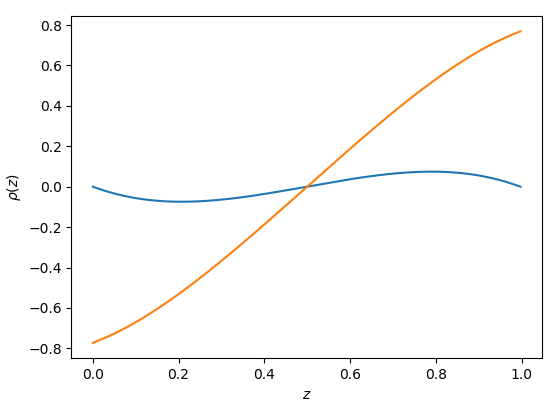
\includegraphics[width=0.8\textwidth]{figures/dirichlet/renormalization_comparison_rho.png}
	\caption{The vacuum polarization at first order in $\lambda$ in Dirichlet boundary conditions. In orange, $\rho$ as calculated using the mode sum in \cite{Ambjorn1983}, and in blue using point splitting with respect to the Hadamard parametrix as in \cite{Wernersson2020}. \note{Here I intend to add a third curve, with the mode sum formula for $\rho$ for $N=1$, which is the one used in \cite{Ambjorn1983}.}}
	\label{fig:perturbative-rho-comparison}
\end{figure}
We show in the figure \ref{fig:perturbative-rho-comparison} the comparison between the two $\rho$. Notice how the addition of the potential term in \eqref{eq:Hadamard-vacuum-polarization} forces $\rho$ to be 0 at the boundaries, as one would expect for Dirichlet boundary conditions. We also observe that the overall vacuum polarization is much stronger when calculating it using the mode sum formula. The main claim in  \cite{Ambjorn1983}, is that when considerring the back reaction of the scalar field, the instabilities that appear in the external field approximation disappear. However, since \cite{Ambjorn1983} uses a wrong expression to calculate the back-reaction of the scalar field, and the correct expression leads to a much 'weaker'  $\rho$, it is not obvious to say whether the back-reaction of the field is enough to raise the energy of the modes enough so as to avoid the original instabilities.
\section{The iterative procedure}

To include backreaction into the calculation, we proceed iteratively.
Following the convention used in \cite{Ambjorn1983}, we label by $\kappa$ each of the iterations. For a given $A_0^{\kappa}$, at each step $\kappa$ we solve numerically the following equations,
\begin{align}
	\partial_1^2 \phi^{\kappa+1}_n &=
	\left( - (\omega^{\kappa+1}_n - \varepsilon A^{\kappa}_0(z))^2 + m^2 \right) \phi^{\kappa+1}_n
	\label{eq:iterative-TIKGE}\\
	\begin{split}
		\varepsilon A_0^{\kappa}(z) &= -\lambda\left( z-\frac{1}{2} \right)  - \varepsilon\int_{\frac{1}{2}}^{z} \int_{0}^{z'} \rho^{\kappa}(z'')  dz'' dz'\\
		\varepsilon A_0^{0}(z) &= -\lambda\left( z-\frac{1}{2}\right) 
	\end{split}
	\label{eq:potential-at-step-kappa}
.
\end{align}
with $\rho$ calculated using \eqref{eq:Hadamard-vacuum-polarization}, up to a finite mode cutoff in the sum. This cutoff at mode N causes the calculated $\rho$ to be oscillatory, of period $\Delta z = \frac{1}{N+1}$, which should be averaged out.

Finally, we take the limit $\kappa \to \infty$, i.e. solve equation \eqref{eq:iterative-TIKGE} for a given potential $A_0^{\kappa}$, calculate the corresponding induced potential at $\kappa$, and solve equation \eqref{eq:iterative-TIKGE} using this new potential. We look for convergence following this procedure. The computation is halted when convergence with respect to some norm is found. Once a self-consistent solution is found, we use this solution as a guess for some new $\lambda$ value, greater than the old one. In this way, we sample the whole $\lambda$-parameter space to study the interaction between the scalar field and the external electric field. 

This procedure can be also be stated in terms of infinite dimensional fixed point problems,
\begin{align}
	A_0 = f(A_0),
\end{align}
with $f$ the update rule given by equation \eqref{eq:potential-at-step-kappa}. The function $f$ has no closed form, as calculating $\rho$ in \eqref{eq:potential-at-step-kappa} involves taking all the steps that were explained throughout this section. 

\subsection{Numerical instabilities}
Even though we are considering the back-reaction of the field, this problem still presents some instabilities when crossing $\lambda\approx \lambda_c$. When sampling the $\lambda$-parameter space, if the step  $\Delta \lambda$ is too big, then one of two things might happen:
\begin{enumerate}
	\item Since we are using the previous solutions as the initial guess to find the self-consistent solution, the screening from the previous solution might not be strong enough causing the energies of some modes to not have solutions in $\mathbb{R}$, or
	\item convergence is too slow.
\end{enumerate}
Even though this can in theory be overcome by choosing smaller $\Delta \lambda$, in practice $\Delta \lambda$ can get to the order of  $10^{-7}$. At $\sim 30s $ per value of $\lambda$, this amounts to about 10 years to  achieve a step of unit size in $\lambda$.

To overcome this, we slightly modify the iterative procedure with a \textit{relaxing} procedure, 
\begin{align}
	A_0^{\kappa+1}(z) = c A_0^{\kappa}(z)+ (1-c) \left[ -\lambda \left( z-\frac{1}{2} \right) - \int_{\frac{1}{2}}^{z} \int_{0}^{z'} \rho^{\kappa} (z'') dz'' dz'   \right], \,\,\, 0< c \lesssim 1.
\end{align}
This scheme avoids these instabilities by allowing self consistent solutions to "relax" into one another, i.e. if for a certain $\lambda$ value a self-consistent solution is found but $\Delta \lambda$ was too big, the change in the potential will not be as strong as it was in the previous scheme. The closer the parameter $c$ is to 1, the slower the convergence, but the more relaxed.

\section{Computational details}

\subsection{Noise filtering}
To solve this problem numerically, we split the interval $(0, 1)$ into M equal intervals, with the mesh points $0<\ldots<z_i<\ldots<1$ and  $i\in \left[ 0, M-1 \right] $.

In the (numerical) computation of \eqref{eq:Hadamard-vacuum-polarization} one needs to cut the mode sum at some finite mode N. This induces oscillations of period $\Delta z = \frac{1}{N + 1}$ in the resulting vacuum polarization, which should be averaged out. To do this, we convolute the resulting $\rho$ with a very specific array, designed to cancel these oscillations out. 
Recall the definition of the convolution of two arrays $\rho_n$, $b_n$ not necessarily of the same length
\begin{align}
	(\rho*b)_n = \sum_{n=0}^{M} \rho_m b_{n-m}.
\end{align}
A convoluting array of the form\footnote{It should be renormalized so that the sum of its elements is 1}
\begin{align}
	b_n = \left[ 1, 0 , 4 , 0 , 6 , 0,4,0,1 \right] 
\end{align}
approximately cancels the oscillations. For this to be effective, this array should "fit" exactly one period of the noise oscillations, and therefore the number of mesh points should be exactly $M = 8 (N + 1)$.

    \section{Results}

\begin{frame}{The energy of the modes for each $\lambda$}
	\begin{figure}[h]
		\centering
		\caption{$\omega_1$ as a function of $\lambda$ for the massless case in the \textbf{external field approximation}.}
		\label{fig:figures-eigenvalue_evolution_a_1_0-png}
		\includegraphics[width=0.6\textwidth]{figures/eigenvalues-external-field-approximation.png}
	\end{figure}
\end{frame}

\begin{frame}{The energy of the modes for each $\lambda$}
\begin{figure}[h]
	\centering
	\caption{$\omega_1$ as a function of $\lambda$ in the mode sum prescription with $N=1$. }
	\label{fig:figures-eigenvalues_ambjorn}
	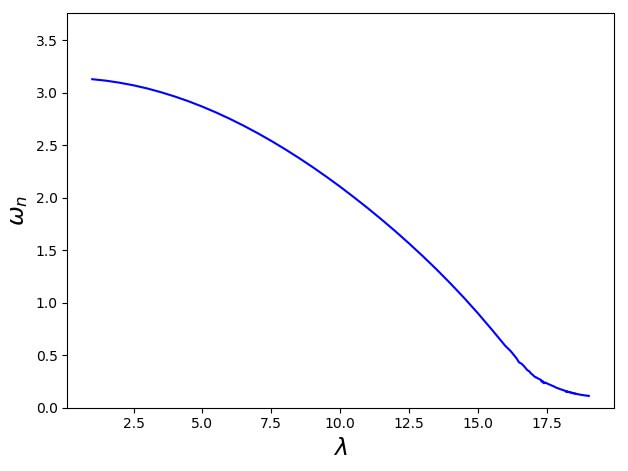
\includegraphics[width=0.6\textwidth]{figures/eigenvalues_ambjorn.png}
\end{figure}
\end{frame}

\begin{frame}{The energy of the modes for each $\lambda$}
\begin{figure}[h]
	\centering
	\caption{The energy of the first three modes of the scalar field in the Hadamard point-splitting prescription with cutoff $N=12$ as $\lambda$ increases.}
	\label{fig:figures-eigenvalue-evolution-png}
	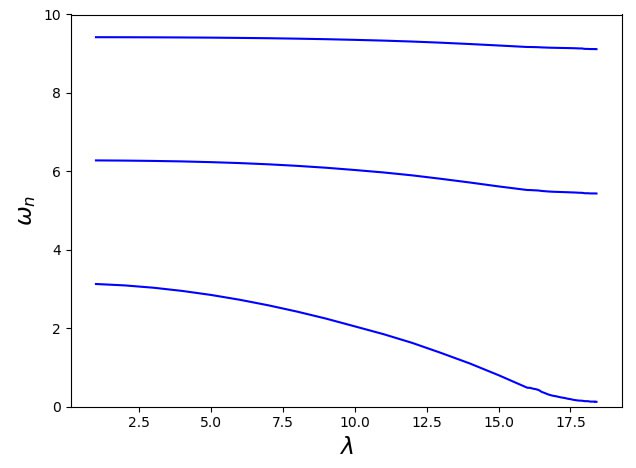
\includegraphics[width=0.5\textwidth]{figures/eigenvalue-evolution.png}
	
\end{figure}
\end{frame}
\begin{frame}{The energy of the modes at each $\lambda$}
\begin{figure}[h]
	\centering
	\caption{$\omega_1$ as a function of $\lambda$ for the \textcolor{blue}{mode sum formula prescription}, \textcolor{orange}{Hadamard point-splitting prescription} and \textcolor{green}{external field approximation}.}
	\label{fig:figures-eigenvalue-evolution-png}
	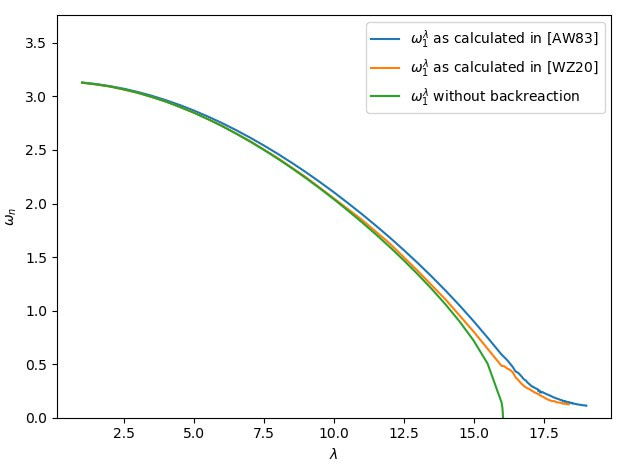
\includegraphics[width=0.5\textwidth]{figures/comparing-energies.png}
	
\end{figure}
\end{frame}


\begin{frame}{Self consistent vacuum polarizations for low $\lambda$}
	\begin{columns}
	    \begin{column}{0.5\textwidth}
	    \begin{figure}[h]
	    	\centering
	    	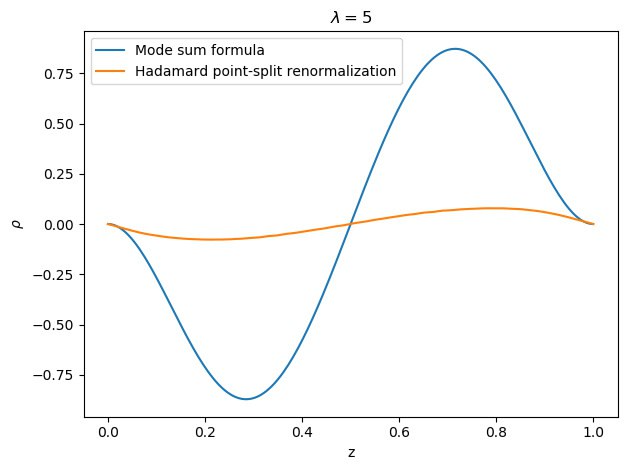
\includegraphics[width=0.8\textwidth]{figures/low-lambda-vacuum-polarization.png}
	    	\caption{$\lambda=5$ comparison of the self consistent vacuum polarization.}
	    	\label{fig:figures-}
	    \end{figure}
	    \end{column}
	    \begin{column}{0.5\textwidth}
	    \begin{figure}[h]
	    	\centering
	    	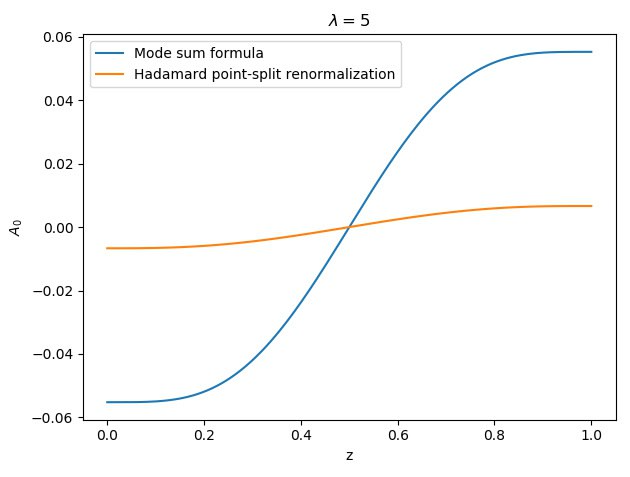
\includegraphics[width=0.8\textwidth]{figures/low-lambda-induced-A0.png}
	    	\caption{$\lambda=5$ comparison of the self consistent induced $A_0$}
	    	\label{fig:figures-}
	    \end{figure}
	    \end{column}
	\end{columns}
\end{frame}
\begin{frame}{Self consistent vacuum polarizations for high $\lambda$}
	\begin{columns}
	    \begin{column}{0.5\textwidth}
	    \begin{figure}[h]
	    	\centering
	    	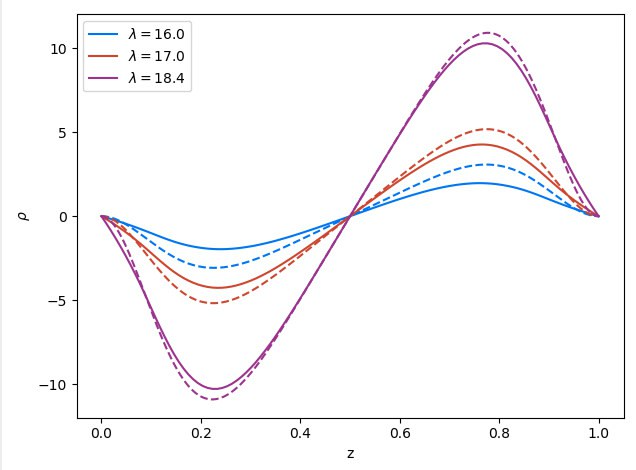
\includegraphics[width=0.8\textwidth]{figures/high-lambda-vacuum-polarization.png}
	    	\caption{Higher values of $\lambda$ comparison of the self consistent vacuum polarization.}
	    	\label{fig:figures-}
	    \end{figure}
	    \end{column}
	    \begin{column}{0.5\textwidth}
	    \begin{figure}[h]
	    	\centering
	    	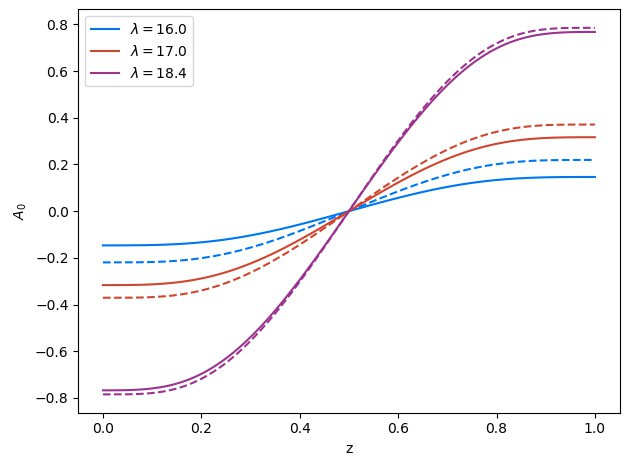
\includegraphics[width=0.8\textwidth]{figures/high-lambda-induced-A0.png}
	    	\caption{Higher values of $\lambda$ comparison of the self consistent vacuum polarization.}
	    	\label{fig:figures-}
	    \end{figure}
	    \end{column}
	\end{columns}
	Dashed lines: mode sum formula. 

	Solid lines: Hadamard point-splitting renormalization.
\end{frame}

\begin{frame}{Vacuum polarization for different $\lambda$}
	\begin{figure}[h]
		\centering
		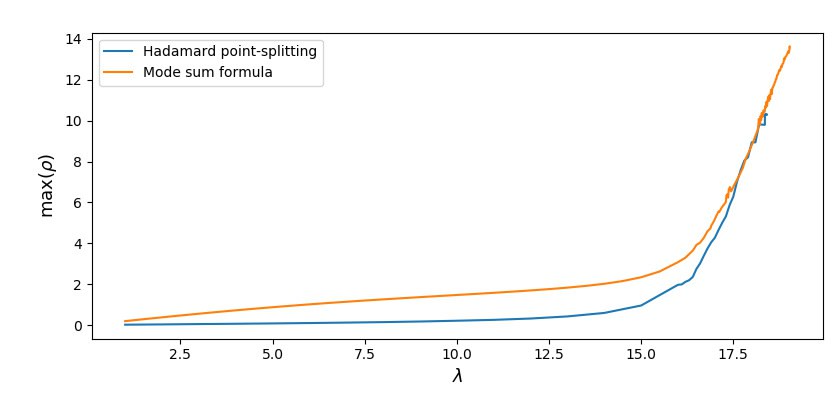
\includegraphics[width=0.8\textwidth]{figures/different-lambda-rho.png}
		\caption{The maximum of the vacuum polarization for different values of the background electric field strength.}
		\label{fig:figures-different-lambda-rho-png}
	\end{figure}
\end{frame}


    \appendix
    \chapter{Computation details}

\section{Numerical methods}
We solve equation \eqref{eq:TIKGE} computationally, using fourth order Runge-Kutta method, and the $\omega_n$ are sought after by using the bisection method, 

\section{Calculating series and limits}

The vacuum polarization \eqref{eq:Hadamard-vacuum-polarization} should be calculated by summing over all modes of the Klein-Gordon field, and then taking the limits $\tau\to 0, \text{and } \epsilon \to 0^+$. To do this compuptationally, first we note that due to the chosen gauge we can state $\omega_n =-\omega_{n}$. This allows us to write equation \eqref{eq:Hadamard-vacuum-polarization} as a single sum, 
\begin{align}
	\begin{split}
			&\rho(z) =  \\
			&\lim_{\tau \to 0}\left(
			\sum_{n> 0}^{}\left[ (\omega_n - A_0) \|\phi_n\|^2   -
		(\omega_{n} + A_0) \|\phi_{-n}\|^2 \right]e^{i \omega_n (\tau + i\varepsilon)}  \right)
			+ \frac{e^2}{\pi} A_0(z).
	\end{split}
\end{align}
Note that this expression is no longer gauge independent.

If the coefficients of the exponential functions decay fast enough as $n$ grows, we can commute the limit and the sum so that 
\begin{align}
	\begin{split}
			\rho(z) =  
			\sum_{n> 0}^{}\left[ (\omega_n - A_0) \|\phi_n\|^2   -
		(\omega_{n} + A_0) \|\phi_{-n}\|^2 \right]
			+ \frac{e^2}{\pi} A_0(z).
	\end{split}
\end{align}

However, we can only calculate a finite amount of mode solutions, so the sum is to be taken only until a certain mode cutoff $N$. This finite cutoff induces oscillations on the calculated vacuum polarization, of period $\Delta z = \frac{1}{N+1}$. These should be averaged out by convoluting the resulting vacuum polarization with a suitable array.

    \chapter{Calculating vacuum polarization at first perturbative order}
In the perturbative approximation, for the massless case
\begin{align}
	\begin{split}
		\omega_n &= n \pi \\
	\phi_n^{D} &= \left( m^2 + \pi^2  n^2 \right)^{-\frac{1}{4}} \Biggl[ \sin\pi n z \\
		   &\left.+ \lambda \frac{\sqrt{m^2 + \pi^2 n^2} }{2 \pi \lvert n \rvert} 
		\left( 
		\frac{1}{\pi n}\left( \frac{1}{2} - z \right) \sin \pi n z - z(1-z) \cos \pi n z \right) 
	\right]  \\
	\phi_n^{D} &= \frac{1}{\sqrt{\pi \lvert n \rvert}}  \Biggl[ \sin\pi n z 
		   \left.+ \frac{\lambda}{2}		\left( 
		\frac{1}{\pi n}\left( \frac{1}{2} - z \right) \sin \pi n z - z(1-z) \cos \pi n z \right) 
	\right] 
	\end{split} 
\end{align}

At first order in $\lambda$, 
\begin{align}
	\lvert \phi_n^{D}\rvert^2 &= \frac{1}{\pi \abs{n}} \Biggl[ \sin^2\pi n z 
		   \left.- \lambda \sin \pi n z		\left( 
		\frac{1}{\pi n}\left( z - \frac{1}{2} \right) \sin \pi n z + z(1-z) \cos \pi n z \right) 
	\right] 
\end{align}

The charge density for the nth mode
\begin{align*}
	(\pi n - \varepsilon A_0)	\lvert \phi_n^{D}\rvert^2 &= (\pi n + \lambda (z-\frac{1}{2}) )\frac{1}{\pi \abs{n}}  \Biggl[ \sin^2\pi n z  \\
									  & \left.+ \lambda \sin \pi n z		\left( 
			\frac{1}{\pi n}\left( \frac{1}{2} - z \right) \sin \pi n z - z(1-z) \cos \pi n z \right) 
		\right]  \\
&= \text{sign}(n)\Biggl[ \sin^2\pi n z  \\
									  & \left.+ \lambda \sin \pi n z		\left( 
			\frac{1}{\pi n}\left( \frac{1}{2} - z \right) \sin \pi n z - z(1-z) \cos \pi n z \right) 
		\right] \\
									  &+\frac{ \lambda \left( z-\frac{1}{2} \right) }{\pi \abs{n} }
\Biggl[ \sin^2\pi n z  \\
									  & \left.+ \lambda \sin \pi n z		\left( 
			\frac{1}{\pi n}\left( \frac{1}{2} - z \right) \sin \pi n z - z(1-z) \cos \pi n z \right) 
		\right] \\
&= \text{sign}(n)\Biggl[ \sin^2\pi n z  \\
									  & \left.+ \lambda \sin \pi n z		\left( 
			\frac{1}{\pi n}\left( \frac{1}{2} - z \right) \sin \pi n z - z(1-z) \cos \pi n z \right) 
		\right] \\
									  &+ \frac{\lambda \left( z-\frac{1}{2} \right)}{\pi \abs{n}}
\sin^2\pi n z  
\end{align*}

And for the -nth mode
\begin{align*}
-(\pi n + \varepsilon A_0)	\lvert \phi_{-n}^{D}\rvert^2
&= -\text{sign}(n)\Biggl[ \sin^2\pi n z  \\
									  & \left.- \lambda \sin \pi n z		\left( 
			\frac{1}{\pi n}\left( \frac{1}{2} - z \right) \sin \pi n z - z(1-z) \cos \pi n z \right) 
		\right] \\
									  &+ \frac{\lambda \left( z-\frac{1}{2} \right)}{\pi \abs{n}}
\sin^2\pi n z  
\end{align*}

So the contribution to the charge density of the $n$th mode is given by 
\begin{align*}
	(\pi n - \varepsilon A_0)	\lvert \phi_{n}^{D}\rvert^2 
	&-(\pi n + \varepsilon A_0)	\lvert \phi_{-n}^{D}\rvert^2 = \\
	& \frac{2 \lambda \sin^2 \pi n z }{\pi n}\left( \frac{1}{2}-z \right)  - 2\lambda z (1-z )\sin \pi n z  \cos \pi n z  \\&+ 2 \frac{\lambda \left( z-\frac{1}{2} \right) }{\pi \abs{n}}\sin ^2 \pi n z
\end{align*}

\begin{align}
\rho(z) = \varepsilon \lim_{\tau\to 0} \sum_{n=1}^{\infty} \left( \lvert \phi_n\rvert ^2 (\pi n - \varepsilon A_0) - \lvert \phi_{-n}\rvert ^2 (\pi n + \varepsilon A_0) \right)  e^{i \pi n (\tau + i \epsilon)} + \frac{e^2}{\pi}A_0.
\end{align}


    \chapter{Calculating vacuum polarization using Hadamard point-splitting renormalization}

The expression for the vacuum polarization comes from the zeroth component of the charge current density 
\begin{align}
	\rho(z) = \vacuum{ \phi^* D_0 \phi - \phi D_0^* \phi^*},
\end{align}
with the field given by its energy mode expansion 
\begin{align}
	\phi(t, z) = \sum_{n>0}^{} a_n \phi_n(z) e ^{-i\omega t} 
	i+ \sum_{n<0}^{} b_n^\dagger \phi_n(z) e ^{-i\omega t} .
\end{align}

Using the Hadamard point-splitting renormalization of the products of (derivaatives of fields) \eqref{eq:point-splitting-wrt-a-Hadamard-parametrix}, from equation \eqref{eq:vacuum-polarization} we need to calculate the two two-point functions $w^{\phi \phi^*}$, $w^{\phi^* \phi}$ and their corresponding Hadamard paramatrices $H^{\phi \phi^*}$, $H^{\phi^* \phi}$.

We are performing the point-splitting in the time direction, $x'= (t + \tau, z)$.
We start by calculating the second term in \eqref{eq:vacuum-polarization}. The relevant two-point function is 
\begin{align}
	w^{\phi\phi^*}(x, x') = \vacuum{  \phi(x)\phi^* (x') } = \sum_{n>0}^{} \abs{\phi_n(z)}^2 e^{i\omega_\tau},
\end{align}
and therefore 
\begin{align}
	D_0^*'
	w^{\phi\phi^*}(x, x') = i\sum_{n>0}^{} (\omega_n - eA_0)\abs{\phi_n(z)}^2 e^{i\omega_\tau}.
\end{align}

The Hadamard parametrix of the two-point function $w^{\phi\phi^*}$ is (up to order relevang for the charge density operator) 
\begin{align}
	H^{\phi \phi^*}= -\frac{1}{4 \pi} U(x, x') \log(\tau^2 + i\varepsilon \tau),
\end{align}
again, with $U(x,x') = \exp\left(ieA_0\tau \right) $. We calculate 
\begin{align}
	\begin{split}
			D_0^*'H^{\phi \phi^*}(x, x')&= -\frac{1}{4\pi} (\partial_0- ieA_0)e^{ieA0\tau} \log\left( \tau^2 + i\varepsilon \tau \right) \\
			&= -\frac{1}{4\pi} ieA_0 e^{ieA_0 \tau} \log(\tau^2+i\varepsilon \tau) 
		-\frac{1}{4\pi} e^{ieA_0 \tau} \frac{2\tau +i \varepsilon }{\tau^2+i\varepsilon\tau} + \frac{1}{4\pi} ieA_0e^{ieA_0\tau} \log(\tau^2+i\varepsilon \tau)\\
		&= -\frac{1}{2\pi}(1+ieA_0\tau) \frac{1}{\tau + i\varepsilon} 
	\end{split}.
\end{align}
Thus, 
\begin{align}
	\vacuum{\phi D_0^*'\phi^*} = \lim_{\tau \to 0} i\sum_{n>0}^{} (\omega_n - eA_0)\abs{\phi_n(z)}^2 e^{i\omega_n (\tau + i \varepsilon)} + \frac{1}{2\pi}(1+ieA_0\tau) \frac{1}{\tau + i\varepsilon} 
\end{align}

In a similar fashion, 
\begin{align}
	D_0'w^{\phi^* \phi}(x, x') = -i \sum_{n<0}^{} \left( \omega_n  -eA_0 \right) \abs{\phi_n}^2 e^{i\omega_n \tau}-\frac{1}{2\pi}(1+ieA_0\tau) \frac{1}{\tau + i\varepsilon},
\end{align}
and 
\begin{align}
	\begin{split}
			D_0'H^{\phi^* \phi}(x, x')&= -\frac{1}{4\pi} (\partial_0+ ieA_0)e^{-ieA0\tau} \log\left( \tau^2 + i\varepsilon \tau \right) \\
			&= \frac{1}{4\pi} ieA_0 e^{-ieA_0 \tau} \log(\tau^2+i\varepsilon \tau) 
		-\frac{1}{4\pi} e^{-ieA_0 \tau} \frac{2\tau +i \varepsilon }{\tau^2+i\varepsilon\tau} - \frac{1}{4\pi} ieA_0e^{-ieA_0\tau} \log(\tau^2+i\varepsilon \tau)\\
		&= -\frac{1}{2\pi}(1-ieA_0\tau) \frac{1}{\tau + i\varepsilon} 
	\end{split}.
\end{align}
The vacuum expectation value of the first term in \eqref{eq:vacuum-polarization} is 
\begin{align}
	\vacuum{\phi^* D_0'\phi} = \lim_{\tau \to 0} -i\sum_{n>0}^{} (\omega_n - eA_0)\abs{\phi_n(z)}^2 e^{i\omega_n (\tau+ i \varepsilon)} + \frac{1}{2\pi}(1-ieA_0\tau) \frac{1}{\tau + i\varepsilon} 
\end{align}

Following equation \eqref{eq:vacuum-polarization}, we subtract these two and multiply by $ie$. The diverging parts cancel out resulting in the following expression for the vacuum polarization
\begin{align}
	\begin{split}
		\rho(z)	 = e\lim_{\varepsilon \to 0^+} \lim_{\tau \to 0}  &\left[  \sum_{n>0}^{} (\omega_n - eA_0)\abs{\phi_n(z)}^2 e^{i\omega_n (\tau+ i \varepsilon)} \right. \\
			   +& \left.  \sum_{n<0}^{} (\omega_n - eA_0)\abs{\phi_n(z)}^2 e^{-i\omega_n (\tau+ i \varepsilon)} \right]  + \frac{e^2}{\pi}A_0(z)\\
	\end{split}
\end{align}



    \bibliographystyle{abbrvnat}
    \bibliography{MyThesis}
\end{document}
